% Options for packages loaded elsewhere
% Options for packages loaded elsewhere
\PassOptionsToPackage{unicode}{hyperref}
\PassOptionsToPackage{hyphens}{url}
\PassOptionsToPackage{dvipsnames,svgnames,x11names}{xcolor}
%
\documentclass[
  letterpaper,
  DIV=11,
  numbers=noendperiod]{scrartcl}
\usepackage{xcolor}
\usepackage[margin=1in]{geometry}
\usepackage{amsmath,amssymb}
\setcounter{secnumdepth}{5}
\usepackage{iftex}
\ifPDFTeX
  \usepackage[T1]{fontenc}
  \usepackage[utf8]{inputenc}
  \usepackage{textcomp} % provide euro and other symbols
\else % if luatex or xetex
  \usepackage{unicode-math} % this also loads fontspec
  \defaultfontfeatures{Scale=MatchLowercase}
  \defaultfontfeatures[\rmfamily]{Ligatures=TeX,Scale=1}
\fi
\usepackage{lmodern}
\ifPDFTeX\else
  % xetex/luatex font selection
  \setmainfont[]{Latin Modern Roman}
  \setsansfont[]{Latin Modern Sans}
  \setmonofont[]{Latin Modern Mono}
\fi
% Use upquote if available, for straight quotes in verbatim environments
\IfFileExists{upquote.sty}{\usepackage{upquote}}{}
\IfFileExists{microtype.sty}{% use microtype if available
  \usepackage[]{microtype}
  \UseMicrotypeSet[protrusion]{basicmath} % disable protrusion for tt fonts
}{}
\makeatletter
\@ifundefined{KOMAClassName}{% if non-KOMA class
  \IfFileExists{parskip.sty}{%
    \usepackage{parskip}
  }{% else
    \setlength{\parindent}{0pt}
    \setlength{\parskip}{6pt plus 2pt minus 1pt}}
}{% if KOMA class
  \KOMAoptions{parskip=half}}
\makeatother
% Make \paragraph and \subparagraph free-standing
\makeatletter
\ifx\paragraph\undefined\else
  \let\oldparagraph\paragraph
  \renewcommand{\paragraph}{
    \@ifstar
      \xxxParagraphStar
      \xxxParagraphNoStar
  }
  \newcommand{\xxxParagraphStar}[1]{\oldparagraph*{#1}\mbox{}}
  \newcommand{\xxxParagraphNoStar}[1]{\oldparagraph{#1}\mbox{}}
\fi
\ifx\subparagraph\undefined\else
  \let\oldsubparagraph\subparagraph
  \renewcommand{\subparagraph}{
    \@ifstar
      \xxxSubParagraphStar
      \xxxSubParagraphNoStar
  }
  \newcommand{\xxxSubParagraphStar}[1]{\oldsubparagraph*{#1}\mbox{}}
  \newcommand{\xxxSubParagraphNoStar}[1]{\oldsubparagraph{#1}\mbox{}}
\fi
\makeatother

\usepackage{color}
\usepackage{fancyvrb}
\newcommand{\VerbBar}{|}
\newcommand{\VERB}{\Verb[commandchars=\\\{\}]}
\DefineVerbatimEnvironment{Highlighting}{Verbatim}{commandchars=\\\{\}}
% Add ',fontsize=\small' for more characters per line
\usepackage{framed}
\definecolor{shadecolor}{RGB}{241,243,245}
\newenvironment{Shaded}{\begin{snugshade}}{\end{snugshade}}
\newcommand{\AlertTok}[1]{\textcolor[rgb]{0.68,0.00,0.00}{#1}}
\newcommand{\AnnotationTok}[1]{\textcolor[rgb]{0.37,0.37,0.37}{#1}}
\newcommand{\AttributeTok}[1]{\textcolor[rgb]{0.40,0.45,0.13}{#1}}
\newcommand{\BaseNTok}[1]{\textcolor[rgb]{0.68,0.00,0.00}{#1}}
\newcommand{\BuiltInTok}[1]{\textcolor[rgb]{0.00,0.23,0.31}{#1}}
\newcommand{\CharTok}[1]{\textcolor[rgb]{0.13,0.47,0.30}{#1}}
\newcommand{\CommentTok}[1]{\textcolor[rgb]{0.37,0.37,0.37}{#1}}
\newcommand{\CommentVarTok}[1]{\textcolor[rgb]{0.37,0.37,0.37}{\textit{#1}}}
\newcommand{\ConstantTok}[1]{\textcolor[rgb]{0.56,0.35,0.01}{#1}}
\newcommand{\ControlFlowTok}[1]{\textcolor[rgb]{0.00,0.23,0.31}{\textbf{#1}}}
\newcommand{\DataTypeTok}[1]{\textcolor[rgb]{0.68,0.00,0.00}{#1}}
\newcommand{\DecValTok}[1]{\textcolor[rgb]{0.68,0.00,0.00}{#1}}
\newcommand{\DocumentationTok}[1]{\textcolor[rgb]{0.37,0.37,0.37}{\textit{#1}}}
\newcommand{\ErrorTok}[1]{\textcolor[rgb]{0.68,0.00,0.00}{#1}}
\newcommand{\ExtensionTok}[1]{\textcolor[rgb]{0.00,0.23,0.31}{#1}}
\newcommand{\FloatTok}[1]{\textcolor[rgb]{0.68,0.00,0.00}{#1}}
\newcommand{\FunctionTok}[1]{\textcolor[rgb]{0.28,0.35,0.67}{#1}}
\newcommand{\ImportTok}[1]{\textcolor[rgb]{0.00,0.46,0.62}{#1}}
\newcommand{\InformationTok}[1]{\textcolor[rgb]{0.37,0.37,0.37}{#1}}
\newcommand{\KeywordTok}[1]{\textcolor[rgb]{0.00,0.23,0.31}{\textbf{#1}}}
\newcommand{\NormalTok}[1]{\textcolor[rgb]{0.00,0.23,0.31}{#1}}
\newcommand{\OperatorTok}[1]{\textcolor[rgb]{0.37,0.37,0.37}{#1}}
\newcommand{\OtherTok}[1]{\textcolor[rgb]{0.00,0.23,0.31}{#1}}
\newcommand{\PreprocessorTok}[1]{\textcolor[rgb]{0.68,0.00,0.00}{#1}}
\newcommand{\RegionMarkerTok}[1]{\textcolor[rgb]{0.00,0.23,0.31}{#1}}
\newcommand{\SpecialCharTok}[1]{\textcolor[rgb]{0.37,0.37,0.37}{#1}}
\newcommand{\SpecialStringTok}[1]{\textcolor[rgb]{0.13,0.47,0.30}{#1}}
\newcommand{\StringTok}[1]{\textcolor[rgb]{0.13,0.47,0.30}{#1}}
\newcommand{\VariableTok}[1]{\textcolor[rgb]{0.07,0.07,0.07}{#1}}
\newcommand{\VerbatimStringTok}[1]{\textcolor[rgb]{0.13,0.47,0.30}{#1}}
\newcommand{\WarningTok}[1]{\textcolor[rgb]{0.37,0.37,0.37}{\textit{#1}}}

\usepackage{longtable,booktabs,array}
\usepackage{calc} % for calculating minipage widths
% Correct order of tables after \paragraph or \subparagraph
\usepackage{etoolbox}
\makeatletter
\patchcmd\longtable{\par}{\if@noskipsec\mbox{}\fi\par}{}{}
\makeatother
% Allow footnotes in longtable head/foot
\IfFileExists{footnotehyper.sty}{\usepackage{footnotehyper}}{\usepackage{footnote}}
\makesavenoteenv{longtable}
\usepackage{graphicx}
\makeatletter
\newsavebox\pandoc@box
\newcommand*\pandocbounded[1]{% scales image to fit in text height/width
  \sbox\pandoc@box{#1}%
  \Gscale@div\@tempa{\textheight}{\dimexpr\ht\pandoc@box+\dp\pandoc@box\relax}%
  \Gscale@div\@tempb{\linewidth}{\wd\pandoc@box}%
  \ifdim\@tempb\p@<\@tempa\p@\let\@tempa\@tempb\fi% select the smaller of both
  \ifdim\@tempa\p@<\p@\scalebox{\@tempa}{\usebox\pandoc@box}%
  \else\usebox{\pandoc@box}%
  \fi%
}
% Set default figure placement to htbp
\def\fps@figure{htbp}
\makeatother





\setlength{\emergencystretch}{3em} % prevent overfull lines

\providecommand{\tightlist}{%
  \setlength{\itemsep}{0pt}\setlength{\parskip}{0pt}}



 


% Colors and section/title styling using KOMA-Script interfaces
\usepackage{xcolor}
\definecolor{sectionblue}{HTML}{2563eb}

% KOMA: headings and title/subtitle colors
\setkomafont{title}{\color{sectionblue}\bfseries\Huge}
\setkomafont{subtitle}{\color{sectionblue}\large}
\setkomafont{section}{\color{sectionblue}\bfseries\Large}
\setkomafont{subsection}{\color{sectionblue}\bfseries\large}

% Code block styling via Shaded redefinition
\usepackage{tcolorbox}
\tcbuselibrary{skins,breakable}
\definecolor{codebg}{HTML}{F0F8FF}
\renewenvironment{Shaded}{%
  \begin{tcolorbox}[%
    enhanced,%
    colback=codebg,%
    colframe=codebg,%
    borderline west={3pt}{0pt}{sectionblue},%
    boxrule=0pt,%
    arc=0pt,%
    boxsep=5pt,%
    left=2mm,%
    right=2mm,%
    top=2mm,%
    bottom=2mm% 
  ]% 
}{%
  \end{tcolorbox}%
}
\KOMAoption{captions}{tableheading}
\makeatletter
\@ifpackageloaded{caption}{}{\usepackage{caption}}
\AtBeginDocument{%
\ifdefined\contentsname
  \renewcommand*\contentsname{Table of contents}
\else
  \newcommand\contentsname{Table of contents}
\fi
\ifdefined\listfigurename
  \renewcommand*\listfigurename{List of Figures}
\else
  \newcommand\listfigurename{List of Figures}
\fi
\ifdefined\listtablename
  \renewcommand*\listtablename{List of Tables}
\else
  \newcommand\listtablename{List of Tables}
\fi
\ifdefined\figurename
  \renewcommand*\figurename{Figure}
\else
  \newcommand\figurename{Figure}
\fi
\ifdefined\tablename
  \renewcommand*\tablename{Table}
\else
  \newcommand\tablename{Table}
\fi
}
\@ifpackageloaded{float}{}{\usepackage{float}}
\floatstyle{ruled}
\@ifundefined{c@chapter}{\newfloat{codelisting}{h}{lop}}{\newfloat{codelisting}{h}{lop}[chapter]}
\floatname{codelisting}{Listing}
\newcommand*\listoflistings{\listof{codelisting}{List of Listings}}
\makeatother
\makeatletter
\makeatother
\makeatletter
\@ifpackageloaded{caption}{}{\usepackage{caption}}
\@ifpackageloaded{subcaption}{}{\usepackage{subcaption}}
\makeatother
\usepackage{bookmark}
\IfFileExists{xurl.sty}{\usepackage{xurl}}{} % add URL line breaks if available
\urlstyle{same}
\hypersetup{
  pdftitle={Fine-Grained Dog Breed Classification: A Deep Learning Approach},
  colorlinks=true,
  linkcolor={blue},
  filecolor={Maroon},
  citecolor={Blue},
  urlcolor={Blue},
  pdfcreator={LaTeX via pandoc}}


\title{Fine-Grained Dog Breed Classification: A Deep Learning Approach}
\usepackage{etoolbox}
\makeatletter
\providecommand{\subtitle}[1]{% add subtitle to \maketitle
  \apptocmd{\@title}{\par {\large #1 \par}}{}{}
}
\makeatother
\subtitle{Building State-of-the-Art CNN Models for 120-Class Visual
Recognition}
\author{}
\date{}
\begin{document}
\maketitle

\renewcommand*\contentsname{Table of contents}
{
\hypersetup{linkcolor=}
\setcounter{tocdepth}{3}
\tableofcontents
}

\section{Project Introduction}\label{project-introduction}

\subsection{What This Project Is
About}\label{what-this-project-is-about}

This project tackles the problem of \textbf{fine-grained image
classification} using \textbf{Convolutional Neural Networks (CNNs)}.
Specifically, I will build a deep learning model to classify images of
dogs into their specific breeds. This is a \textbf{multi-class
classification problem} with 120 different dog breed categories.

The architecture approach will utilize \textbf{transfer learning with
pre-trained CNN models} trained on ImageNet. I will implement and
compare multiple architectures:

\begin{enumerate}
\def\labelenumi{\arabic{enumi}.}
\tightlist
\item
  \textbf{Transfer Learning Approach}: Use pre-trained models (ResNet50,
  VGG16, or EfficientNetB0) as feature extractors, freeze the
  convolutional base, and train only the new fully connected
  classification layers on the dog breed dataset
\item
  \textbf{Fine-Tuning Approach}: Start with pre-trained weights, then
  unfreeze some of the top convolutional layers and fine-tune them along
  with the classification layers using a low learning rate
\item
  \textbf{Custom CNN Architecture}: Build a CNN from scratch with
  multiple convolutional blocks (Conv2D + BatchNormalization +
  MaxPooling + Dropout) to serve as a baseline for comparison
\end{enumerate}

I will compare these approaches to determine which strategy yields the
best performance for this specific classification task.

\subsection{Goal and Motivation}\label{goal-and-motivation}

\textbf{Goal}: To develop an accurate deep learning classifier that can
identify dog breeds from images with high precision, and to understand
which architectural approach works best for fine-grained visual
recognition.

\textbf{Why This Matters}:

\begin{itemize}
\tightlist
\item
  \textbf{Practical Application}: Automated breed identification can
  help in animal shelters, veterinary clinics, and pet adoption services
  where quick and accurate breed identification is essential
\item
  \textbf{Lost Pet Recovery}: Can assist in matching found dogs with
  lost pet reports
\item
  \textbf{Education}: Helps dog enthusiasts and potential pet owners
  learn about different breeds
\item
  \textbf{Technical Challenge}: Dog breed classification is a
  challenging fine-grained visual recognition problem because many
  breeds share similar physical characteristics (facial features, body
  shape, coat patterns), making it an excellent testbed for evaluating
  deep learning techniques and transfer learning strategies
\end{itemize}

\textbf{What I Want to Achieve}:

\begin{itemize}
\tightlist
\item
  Build a model that can accurately distinguish between 120 dog breeds,
  even when breeds look visually similar (e.g., Siberian Husky
  vs.~Alaskan Malamute)
\item
  Compare the effectiveness of transfer learning versus training from
  scratch
\item
  Understand which visual features the model uses to make distinctions
  through visualization techniques (such as class activation maps)
\item
  Achieve practical accuracy that could be deployed in real-world
  applications
\end{itemize}

\begin{center}\rule{0.5\linewidth}{0.5pt}\end{center}

\textbf{Expected Outcomes}: A trained CNN model with \textgreater80\%
accuracy on the test set, comprehensive comparison of different
architectures, and insights into what makes certain breeds easier or
harder to classify.

\subsection{Hardware Requirements \& Cost
Considerations}\label{hardware-requirements-cost-considerations}

Deep learning for image classification is \textbf{compute-intensive} and
requires GPU acceleration for practical training times.

\subsubsection{Hardware Requirements}\label{hardware-requirements}

\textbf{GPU (Essential)}: - \textbf{Minimum}: NVIDIA GPU with 8GB+ VRAM
- \textbf{Recommended}: 16GB+ VRAM (A40, A100, RTX 3090/4090) - Training
on CPU would take 50-100× longer (days instead of hours)

\subsubsection{Training Costs (RunPod Cloud
GPU)}\label{training-costs-runpod-cloud-gpu}

\textbf{Current Setup}: 1× NVIDIA A40 (46GB)

\begin{longtable}[]{@{}lll@{}}
\toprule\noalign{}
Training Stage & Time & Cost \\
\midrule\noalign{}
\endhead
\bottomrule\noalign{}
\endlastfoot
Frozen baseline (completed) & 48 min & \$0.32 \\
Fine-tuning unfrozen (next) & 3-5 hours & \$1.50-2.00 \\
Full project & 5-10 hours & \$2-5 \\
\end{longtable}

\textbf{GPU Upgrade Options}: - \textbf{A40}: \$0.40-0.60/hour (current,
baseline performance) - \textbf{H100}: \$2.50-4.00/hour (3-4× faster -
good for rapid iteration) - \textbf{2× A40}: \$0.80-1.20/hour (parallel
training - good for testing multiple models)

\section{Data Loading \& Initial
Inspection}\label{data-loading-initial-inspection}

\subsection{Dataset: Stanford Dogs}\label{dataset-stanford-dogs}

\textbf{Source}: Stanford Dogs Dataset\\
\textbf{URL}: http://vision.stanford.edu/aditya86/ImageNetDogs/\\
\textbf{License}: Academic/Research use\\
\textbf{Size}: \textasciitilde750MB (images), 20,580 total images

\textbf{Dataset Description}:

The Stanford Dogs dataset contains images of 120 breeds of dogs from
around the world. This dataset has been built using images and
annotation from ImageNet for the task of fine-grained image
categorization.

\textbf{Key Statistics}:

\begin{itemize}
\tightlist
\item
  \textbf{120 dog breed classes} (Chihuahua, Afghan\_hound,
  Maltese\_dog, Golden\_retriever, etc.)
\item
  \textbf{20,580 images total} (after validation)
\item
  \textbf{Average 171.5 images per breed} (range: 148-252)
\item
  \textbf{Average image dimensions}: 443×386 pixels
\item
  \textbf{Image format}: JPEG (20,579 images), PNG (1 image)
\item
  \textbf{Color mode}: RGB (20,579 images), RGBA (1 image)
\end{itemize}

\textbf{Data Organization}:

Images are organized in directories by breed:

\begin{verbatim}
data/raw/Images/
├── n02085620-Chihuahua/
├── n02085782-Japanese_spaniel/
├── n02085936-Maltese_dog/
└── ... (120 breed directories total)
\end{verbatim}

\textbf{Preprocessing Pipeline}:

\begin{enumerate}
\def\labelenumi{\arabic{enumi}.}
\tightlist
\item
  \textbf{Download} (\texttt{python\ -m\ dbc.ingest}): Downloaded
  images, annotations, and breed mapping
\item
  \textbf{Validation} (\texttt{python\ -m\ dbc.preprocess}): Scanned all
  20,580 images, validated for corruption, size, and format
\item
  \textbf{Cleaning}: Removed 0 corrupt images, all images passed
  validation ✓
\item
  \textbf{Splitting}: Created stratified 80/20 train/validation split

  \begin{itemize}
  \tightlist
  \item
    Train: 16,508 images
  \item
    Validation: 4,072 images
  \end{itemize}
\end{enumerate}

\textbf{Why This Dataset?}:

\begin{itemize}
\tightlist
\item
  \textbf{Fine-grained classification challenge}: Many breeds share
  similar visual features, making this an excellent test for CNN
  architectures
\item
  \textbf{Sufficient data}: \textasciitilde170 images per class enables
  meaningful training with data augmentation
\item
  \textbf{Real-world applicability}: Breed identification has practical
  uses in animal shelters, veterinary clinics, and pet services
\end{itemize}

\textbf{Dataset Challenges}:

This dataset presents several real-world complications that make
classification more challenging:

\begin{itemize}
\tightlist
\item
  \textbf{Multiple Objects}: Many images contain humans, other animals,
  or various background objects alongside the dogs
\item
  \textbf{Variable Composition}: Dogs may occupy only a small portion of
  the image frame
\item
  \textbf{Background Clutter}: Complex backgrounds with furniture,
  outdoor scenery, or other distractions
\item
  \textbf{Occlusion}: Dogs may be partially hidden or cropped in some
  images
\end{itemize}

These challenges make the task more realistic and require the model to
learn discriminative breed features despite visual noise.

\begin{Shaded}
\begin{Highlighting}[]
\ImportTok{import}\NormalTok{ sys}
\ImportTok{from}\NormalTok{ pathlib }\ImportTok{import}\NormalTok{ Path}
\NormalTok{sys.path.append(}\BuiltInTok{str}\NormalTok{(Path.cwd().parent }\OperatorTok{/} \StringTok{"src"}\NormalTok{))}

\ImportTok{import}\NormalTok{ pandas }\ImportTok{as}\NormalTok{ pd}
\ImportTok{import}\NormalTok{ numpy }\ImportTok{as}\NormalTok{ np}
\ImportTok{import}\NormalTok{ matplotlib.pyplot }\ImportTok{as}\NormalTok{ plt}
\ImportTok{from}\NormalTok{ PIL }\ImportTok{import}\NormalTok{ Image}
\ImportTok{from}\NormalTok{ IPython.display }\ImportTok{import}\NormalTok{ display}
\ImportTok{import}\NormalTok{ json}

\CommentTok{\# Load breed mapping}
\NormalTok{breeds\_df }\OperatorTok{=}\NormalTok{ pd.read\_csv(}\StringTok{"../data/raw/breed\_mapping.csv"}\NormalTok{)}
\BuiltInTok{print}\NormalTok{(}\StringTok{"Breed Mapping (first 10 breeds):"}\NormalTok{)}
\NormalTok{display(breeds\_df.head(}\DecValTok{10}\NormalTok{))}

\CommentTok{\# Load train/val metadata}
\NormalTok{train\_df }\OperatorTok{=}\NormalTok{ pd.read\_csv(}\StringTok{"../artifacts/train\_metadata.csv"}\NormalTok{)}
\NormalTok{val\_df }\OperatorTok{=}\NormalTok{ pd.read\_csv(}\StringTok{"../artifacts/val\_metadata.csv"}\NormalTok{)}

\BuiltInTok{print}\NormalTok{(}\SpecialStringTok{f"}\CharTok{\textbackslash{}n}\SpecialStringTok{Train set: }\SpecialCharTok{\{}\BuiltInTok{len}\NormalTok{(train\_df)}\SpecialCharTok{\}}\SpecialStringTok{ images"}\NormalTok{)}
\BuiltInTok{print}\NormalTok{(}\SpecialStringTok{f"Validation set: }\SpecialCharTok{\{}\BuiltInTok{len}\NormalTok{(val\_df)}\SpecialCharTok{\}}\SpecialStringTok{ images"}\NormalTok{)}

\CommentTok{\# Load dataset statistics}
\ControlFlowTok{with} \BuiltInTok{open}\NormalTok{(}\StringTok{"../artifacts/dataset\_stats.json"}\NormalTok{, }\StringTok{"r"}\NormalTok{) }\ImportTok{as}\NormalTok{ f:}
\NormalTok{    stats }\OperatorTok{=}\NormalTok{ json.load(f)}
    
\BuiltInTok{print}\NormalTok{(}\StringTok{"}\CharTok{\textbackslash{}n}\StringTok{Dataset Statistics:"}\NormalTok{)}
\ControlFlowTok{for}\NormalTok{ key, value }\KeywordTok{in}\NormalTok{ stats.items():}
    \ControlFlowTok{if}\NormalTok{ key }\KeywordTok{not} \KeywordTok{in}\NormalTok{ [}\StringTok{\textquotesingle{}image\_modes\textquotesingle{}}\NormalTok{, }\StringTok{\textquotesingle{}image\_formats\textquotesingle{}}\NormalTok{]:}
        \BuiltInTok{print}\NormalTok{(}\SpecialStringTok{f"  }\SpecialCharTok{\{}\NormalTok{key}\SpecialCharTok{\}}\SpecialStringTok{: }\SpecialCharTok{\{}\NormalTok{value}\SpecialCharTok{\}}\SpecialStringTok{"}\NormalTok{)}
        
\BuiltInTok{print}\NormalTok{(}\StringTok{"}\CharTok{\textbackslash{}n}\StringTok{Train metadata (first 5 samples):"}\NormalTok{)}
\NormalTok{display(train\_df[[}\StringTok{\textquotesingle{}breed\_name\textquotesingle{}}\NormalTok{, }\StringTok{\textquotesingle{}class\_id\textquotesingle{}}\NormalTok{, }\StringTok{\textquotesingle{}width\textquotesingle{}}\NormalTok{, }\StringTok{\textquotesingle{}height\textquotesingle{}}\NormalTok{, }\StringTok{\textquotesingle{}filename\textquotesingle{}}\NormalTok{]].head())}
\end{Highlighting}
\end{Shaded}

\begin{verbatim}
Breed Mapping (first 10 breeds):
\end{verbatim}

\begin{longtable}[]{@{}llll@{}}
\toprule\noalign{}
& class\_id & breed\_name & breed\_dir \\
\midrule\noalign{}
\endhead
\bottomrule\noalign{}
\endlastfoot
0 & 1 & Chihuahua & n02085620-Chihuahua \\
1 & 2 & Japanese\_spaniel & n02085782-Japanese\_spaniel \\
2 & 3 & Maltese\_dog & n02085936-Maltese\_dog \\
3 & 4 & Pekinese & n02086079-Pekinese \\
4 & 5 & Shih-Tzu & n02086240-Shih-Tzu \\
5 & 6 & Blenheim\_spaniel & n02086646-Blenheim\_spaniel \\
6 & 7 & papillon & n02086910-papillon \\
7 & 8 & toy\_terrier & n02087046-toy\_terrier \\
8 & 9 & Rhodesian\_ridgeback & n02087394-Rhodesian\_ridgeback \\
9 & 10 & Afghan\_hound & n02088094-Afghan\_hound \\
\end{longtable}

\begin{verbatim}

Train set: 16508 images
Validation set: 4072 images

Dataset Statistics:
  total_images: 20580
  total_breeds: 120
  avg_images_per_breed: 171.5
  min_images_per_breed: 148
  max_images_per_breed: 252
  avg_width: 442.5318756073858
  avg_height: 385.8612244897959
  avg_size_kb: 36.90375502042335

Train metadata (first 5 samples):
\end{verbatim}

\begin{longtable}[]{@{}llllll@{}}
\toprule\noalign{}
& breed\_name & class\_id & width & height & filename \\
\midrule\noalign{}
\endhead
\bottomrule\noalign{}
\endlastfoot
0 & Afghan\_hound & 10 & 489 & 500 & n02088094\_294.jpg \\
1 & Afghan\_hound & 10 & 500 & 375 & n02088094\_173.jpg \\
2 & Afghan\_hound & 10 & 459 & 500 & n02088094\_4635.jpg \\
3 & Afghan\_hound & 10 & 340 & 500 & n02088094\_515.jpg \\
4 & Afghan\_hound & 10 & 500 & 333 & n02088094\_4072.jpg \\
\end{longtable}

\section{Preprocess}\label{preprocess}

\subsection{Data Cleaning}\label{data-cleaning}

Before training our CNN model, we need to ensure our dataset is clean
and ready. This section analyzes the raw scanned data and applies
quality filters to remove problematic images.

\textbf{Cleaning Checks Performed:}

\begin{enumerate}
\def\labelenumi{\arabic{enumi}.}
\tightlist
\item
  \textbf{Corrupt Image Detection} - Identify images that cannot be
  loaded or have invalid pixel data
\item
  \textbf{Duplicate Removal} - Find and remove duplicate filenames to
  prevent data leakage
\item
  \textbf{Size Validation} - Filter out images that are too small
  (\textless50×50px) or too large (\textgreater10MB)
\item
  \textbf{Color Mode Analysis} - Check for grayscale/RGBA images that
  need RGB conversion
\item
  \textbf{Aspect Ratio Check} - Flag extreme aspect ratios that may
  cause issues during resizing
\end{enumerate}

\textbf{Why This Matters:}

\begin{itemize}
\tightlist
\item
  \textbf{Prevents training crashes} - Ensures all images can be loaded
  successfully
\item
  \textbf{Improves data quality} - Removes low-quality or problematic
  images
\item
  \textbf{Avoids data leakage} - Duplicate removal prevents the same
  image appearing in train and validation
\item
  \textbf{Informs preprocessing} - Understanding color modes and aspect
  ratios helps design the data pipeline
\end{itemize}

\begin{Shaded}
\begin{Highlighting}[]
\CommentTok{\# Load the raw scan results to show cleaning process}
\NormalTok{scan\_df }\OperatorTok{=}\NormalTok{ pd.read\_csv(}\StringTok{"../artifacts/dataset\_scan.csv"}\NormalTok{)}

\BuiltInTok{print}\NormalTok{(}\StringTok{"Data Cleaning Pipeline"}\NormalTok{)}
\BuiltInTok{print}\NormalTok{(}\StringTok{"="}\OperatorTok{*}\DecValTok{60}\NormalTok{)}

\CommentTok{\# Step 1: Check for invalid/corrupt images}
\NormalTok{invalid\_images }\OperatorTok{=}\NormalTok{ scan\_df[scan\_df[}\StringTok{\textquotesingle{}valid\textquotesingle{}}\NormalTok{] }\OperatorTok{==} \VariableTok{False}\NormalTok{]}
\BuiltInTok{print}\NormalTok{(}\SpecialStringTok{f"}\CharTok{\textbackslash{}n}\SpecialStringTok{1. Invalid/Corrupt Images: }\SpecialCharTok{\{}\BuiltInTok{len}\NormalTok{(invalid\_images)}\SpecialCharTok{\}}\SpecialStringTok{"}\NormalTok{)}
\ControlFlowTok{if} \BuiltInTok{len}\NormalTok{(invalid\_images) }\OperatorTok{\textgreater{}} \DecValTok{0}\NormalTok{:}
    \BuiltInTok{print}\NormalTok{(}\StringTok{"   Errors found:"}\NormalTok{)}
    \ControlFlowTok{for}\NormalTok{ \_, row }\KeywordTok{in}\NormalTok{ invalid\_images.head(}\DecValTok{5}\NormalTok{).iterrows():}
        \BuiltInTok{print}\NormalTok{(}\SpecialStringTok{f"     {-} }\SpecialCharTok{\{}\NormalTok{row[}\StringTok{\textquotesingle{}filename\textquotesingle{}}\NormalTok{]}\SpecialCharTok{\}}\SpecialStringTok{: }\SpecialCharTok{\{}\NormalTok{row[}\StringTok{\textquotesingle{}error\textquotesingle{}}\NormalTok{]}\SpecialCharTok{\}}\SpecialStringTok{"}\NormalTok{)}
\ControlFlowTok{else}\NormalTok{:}
    \BuiltInTok{print}\NormalTok{(}\StringTok{"   ✓ No corrupt images detected"}\NormalTok{)}

\CommentTok{\# Step 2: Check for duplicates}
\NormalTok{duplicates }\OperatorTok{=}\NormalTok{ scan\_df[scan\_df.duplicated(subset}\OperatorTok{=}\NormalTok{[}\StringTok{\textquotesingle{}filename\textquotesingle{}}\NormalTok{], keep}\OperatorTok{=}\VariableTok{False}\NormalTok{)]}
\BuiltInTok{print}\NormalTok{(}\SpecialStringTok{f"}\CharTok{\textbackslash{}n}\SpecialStringTok{2. Duplicate Files: }\SpecialCharTok{\{}\BuiltInTok{len}\NormalTok{(duplicates)}\SpecialCharTok{\}}\SpecialStringTok{"}\NormalTok{)}
\ControlFlowTok{if} \BuiltInTok{len}\NormalTok{(duplicates) }\OperatorTok{\textgreater{}} \DecValTok{0}\NormalTok{:}
    \BuiltInTok{print}\NormalTok{(}\SpecialStringTok{f"   Found }\SpecialCharTok{\{}\BuiltInTok{len}\NormalTok{(duplicates)}\SpecialCharTok{\}}\SpecialStringTok{ duplicate filenames"}\NormalTok{)}
\ControlFlowTok{else}\NormalTok{:}
    \BuiltInTok{print}\NormalTok{(}\StringTok{"   ✓ No duplicates found"}\NormalTok{)}

\CommentTok{\# Step 3: Size violations}
\NormalTok{size\_violations }\OperatorTok{=}\NormalTok{ scan\_df[}
\NormalTok{    (scan\_df[}\StringTok{\textquotesingle{}width\textquotesingle{}}\NormalTok{] }\OperatorTok{\textless{}} \DecValTok{50}\NormalTok{) }\OperatorTok{|} 
\NormalTok{    (scan\_df[}\StringTok{\textquotesingle{}height\textquotesingle{}}\NormalTok{] }\OperatorTok{\textless{}} \DecValTok{50}\NormalTok{) }\OperatorTok{|} 
\NormalTok{    (scan\_df[}\StringTok{\textquotesingle{}size\_kb\textquotesingle{}}\NormalTok{] }\OperatorTok{\textgreater{}} \DecValTok{10000}\NormalTok{)}
\NormalTok{]}
\BuiltInTok{print}\NormalTok{(}\SpecialStringTok{f"}\CharTok{\textbackslash{}n}\SpecialStringTok{3. Size Violations: }\SpecialCharTok{\{}\BuiltInTok{len}\NormalTok{(size\_violations)}\SpecialCharTok{\}}\SpecialStringTok{"}\NormalTok{)}
\BuiltInTok{print}\NormalTok{(}\SpecialStringTok{f"   {-} Too small (\textless{}50px): }\SpecialCharTok{\{}\BuiltInTok{len}\NormalTok{(scan\_df[(scan\_df[}\StringTok{\textquotesingle{}width\textquotesingle{}}\NormalTok{] }\OperatorTok{\textless{}} \DecValTok{50}\NormalTok{) }\OperatorTok{|}\NormalTok{ (scan\_df[}\StringTok{\textquotesingle{}height\textquotesingle{}}\NormalTok{] }\OperatorTok{\textless{}} \DecValTok{50}\NormalTok{)])}\SpecialCharTok{\}}\SpecialStringTok{"}\NormalTok{)}
\BuiltInTok{print}\NormalTok{(}\SpecialStringTok{f"   {-} Too large (\textgreater{}10MB): }\SpecialCharTok{\{}\BuiltInTok{len}\NormalTok{(scan\_df[scan\_df[}\StringTok{\textquotesingle{}size\_kb\textquotesingle{}}\NormalTok{] }\OperatorTok{\textgreater{}} \DecValTok{10000}\NormalTok{])}\SpecialCharTok{\}}\SpecialStringTok{"}\NormalTok{)}
\ControlFlowTok{if} \BuiltInTok{len}\NormalTok{(size\_violations) }\OperatorTok{==} \DecValTok{0}\NormalTok{:}
    \BuiltInTok{print}\NormalTok{(}\StringTok{"   ✓ All images meet size requirements"}\NormalTok{)}

\CommentTok{\# Step 4: Color mode check}
\BuiltInTok{print}\NormalTok{(}\SpecialStringTok{f"}\CharTok{\textbackslash{}n}\SpecialStringTok{4. Color Modes:"}\NormalTok{)}
\NormalTok{color\_modes }\OperatorTok{=}\NormalTok{ scan\_df[}\StringTok{\textquotesingle{}mode\textquotesingle{}}\NormalTok{].value\_counts()}
\ControlFlowTok{for}\NormalTok{ mode, count }\KeywordTok{in}\NormalTok{ color\_modes.items():}
    \BuiltInTok{print}\NormalTok{(}\SpecialStringTok{f"   {-} }\SpecialCharTok{\{}\NormalTok{mode}\SpecialCharTok{\}}\SpecialStringTok{: }\SpecialCharTok{\{}\NormalTok{count}\SpecialCharTok{\}}\SpecialStringTok{ images"}\NormalTok{)}
\NormalTok{non\_rgb }\OperatorTok{=}\NormalTok{ scan\_df[scan\_df[}\StringTok{\textquotesingle{}mode\textquotesingle{}}\NormalTok{] }\OperatorTok{!=} \StringTok{\textquotesingle{}RGB\textquotesingle{}}\NormalTok{]}
\BuiltInTok{print}\NormalTok{(}\SpecialStringTok{f"   Note: }\SpecialCharTok{\{}\BuiltInTok{len}\NormalTok{(non\_rgb)}\SpecialCharTok{\}}\SpecialStringTok{ non{-}RGB images will be converted during training"}\NormalTok{)}
\end{Highlighting}
\end{Shaded}

\begin{verbatim}
Data Cleaning Pipeline
============================================================

1. Invalid/Corrupt Images: 0
   ✓ No corrupt images detected

2. Duplicate Files: 0
   ✓ No duplicates found

3. Size Violations: 0
   - Too small (<50px): 0
   - Too large (>10MB): 0
   ✓ All images meet size requirements

4. Color Modes:
   - RGB: 20579 images
   - RGBA: 1 images
   Note: 1 non-RGB images will be converted during training
\end{verbatim}

\begin{Shaded}
\begin{Highlighting}[]
\CommentTok{\# Show the one non{-}RGB image}
\ControlFlowTok{if} \BuiltInTok{len}\NormalTok{(non\_rgb) }\OperatorTok{\textgreater{}} \DecValTok{0}\NormalTok{:}
\NormalTok{    img\_path }\OperatorTok{=}\NormalTok{ Path(}\StringTok{".."}\NormalTok{) }\OperatorTok{/}\NormalTok{ non\_rgb.iloc[}\DecValTok{0}\NormalTok{][}\StringTok{\textquotesingle{}absolute\_path\textquotesingle{}}\NormalTok{]}
\NormalTok{    img }\OperatorTok{=}\NormalTok{ Image.}\BuiltInTok{open}\NormalTok{(img\_path)}
\NormalTok{    plt.figure(figsize}\OperatorTok{=}\NormalTok{(}\DecValTok{6}\NormalTok{, }\DecValTok{6}\NormalTok{))}
\NormalTok{    plt.imshow(img)}
\NormalTok{    plt.title(}\SpecialStringTok{f"Non{-}RGB Image: }\SpecialCharTok{\{}\NormalTok{non\_rgb}\SpecialCharTok{.}\NormalTok{iloc[}\DecValTok{0}\NormalTok{][}\StringTok{\textquotesingle{}mode\textquotesingle{}}\NormalTok{]}\SpecialCharTok{\}}\SpecialStringTok{ mode}\CharTok{\textbackslash{}n}\SpecialCharTok{\{}\NormalTok{non\_rgb}\SpecialCharTok{.}\NormalTok{iloc[}\DecValTok{0}\NormalTok{][}\StringTok{\textquotesingle{}filename\textquotesingle{}}\NormalTok{]}\SpecialCharTok{\}}\SpecialStringTok{"}\NormalTok{)}
\NormalTok{    plt.axis(}\StringTok{\textquotesingle{}off\textquotesingle{}}\NormalTok{)}
\NormalTok{    plt.tight\_layout()}
\NormalTok{    plt.show()}
    
    \BuiltInTok{print}\NormalTok{(}\SpecialStringTok{f"}\CharTok{\textbackslash{}n}\SpecialStringTok{   Decision: The 1 RGBA image will be automatically converted to RGB"}\NormalTok{)}
    \BuiltInTok{print}\NormalTok{(}\SpecialStringTok{f"   during data loading (see data\_loader.py). No manual fixing needed."}\NormalTok{)}
    \BuiltInTok{print}\NormalTok{(}\SpecialStringTok{f"   This is better than modifying raw data files."}\NormalTok{)}
\end{Highlighting}
\end{Shaded}

\pandocbounded{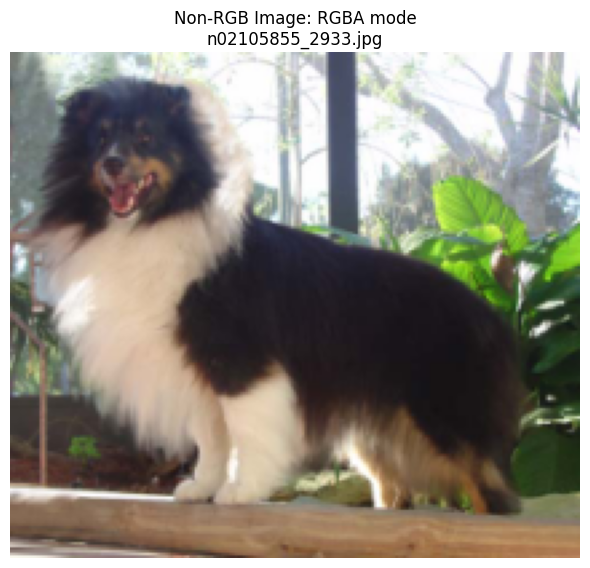
\includegraphics[keepaspectratio]{main_files/figure-pdf/cell-4-output-1.png}}

\begin{verbatim}

   Decision: The 1 RGBA image will be automatically converted to RGB
   during data loading (see data_loader.py). No manual fixing needed.
   This is better than modifying raw data files.
\end{verbatim}

\begin{Shaded}
\begin{Highlighting}[]
\CommentTok{\# Step 5: Extreme aspect ratios}
\NormalTok{scan\_df[}\StringTok{\textquotesingle{}aspect\_ratio\textquotesingle{}}\NormalTok{] }\OperatorTok{=}\NormalTok{ scan\_df[}\StringTok{\textquotesingle{}width\textquotesingle{}}\NormalTok{] }\OperatorTok{/}\NormalTok{ scan\_df[}\StringTok{\textquotesingle{}height\textquotesingle{}}\NormalTok{]}
\NormalTok{extreme\_ratios }\OperatorTok{=}\NormalTok{ scan\_df[}
\NormalTok{    (scan\_df[}\StringTok{\textquotesingle{}aspect\_ratio\textquotesingle{}}\NormalTok{] }\OperatorTok{\textless{}} \FloatTok{0.2}\NormalTok{) }\OperatorTok{|} 
\NormalTok{    (scan\_df[}\StringTok{\textquotesingle{}aspect\_ratio\textquotesingle{}}\NormalTok{] }\OperatorTok{\textgreater{}} \FloatTok{5.0}\NormalTok{)}
\NormalTok{]}
\BuiltInTok{print}\NormalTok{(}\SpecialStringTok{f"}\CharTok{\textbackslash{}n}\SpecialStringTok{5. Extreme Aspect Ratios (\textless{}0.2 or \textgreater{}5.0): }\SpecialCharTok{\{}\BuiltInTok{len}\NormalTok{(extreme\_ratios)}\SpecialCharTok{\}}\SpecialStringTok{"}\NormalTok{)}
\ControlFlowTok{if} \BuiltInTok{len}\NormalTok{(extreme\_ratios) }\OperatorTok{\textgreater{}} \DecValTok{0}\NormalTok{:}
    \BuiltInTok{print}\NormalTok{(}\StringTok{"   Images with unusual ratios (may need special handling):"}\NormalTok{)}
    \ControlFlowTok{for}\NormalTok{ \_, row }\KeywordTok{in}\NormalTok{ extreme\_ratios.head(}\DecValTok{3}\NormalTok{).iterrows():}
        \BuiltInTok{print}\NormalTok{(}\SpecialStringTok{f"     {-} }\SpecialCharTok{\{}\NormalTok{row[}\StringTok{\textquotesingle{}filename\textquotesingle{}}\NormalTok{]}\SpecialCharTok{\}}\SpecialStringTok{: }\SpecialCharTok{\{}\NormalTok{row[}\StringTok{\textquotesingle{}aspect\_ratio\textquotesingle{}}\NormalTok{]}\SpecialCharTok{:.2f\}}\SpecialStringTok{"}\NormalTok{)}

\CommentTok{\# Final summary}
\BuiltInTok{print}\NormalTok{(}\StringTok{"}\CharTok{\textbackslash{}n}\StringTok{"} \OperatorTok{+} \StringTok{"="}\OperatorTok{*}\DecValTok{60}\NormalTok{)}
\BuiltInTok{print}\NormalTok{(}\StringTok{"CLEANING SUMMARY"}\NormalTok{)}
\BuiltInTok{print}\NormalTok{(}\StringTok{"="}\OperatorTok{*}\DecValTok{60}\NormalTok{)}
\NormalTok{clean\_count }\OperatorTok{=} \BuiltInTok{len}\NormalTok{(scan\_df[scan\_df[}\StringTok{\textquotesingle{}valid\textquotesingle{}}\NormalTok{] }\OperatorTok{==} \VariableTok{True}\NormalTok{])}
\NormalTok{removed }\OperatorTok{=} \BuiltInTok{len}\NormalTok{(scan\_df) }\OperatorTok{{-}}\NormalTok{ clean\_count}
\BuiltInTok{print}\NormalTok{(}\SpecialStringTok{f"Initial images:    }\SpecialCharTok{\{}\BuiltInTok{len}\NormalTok{(scan\_df)}\SpecialCharTok{\}}\SpecialStringTok{"}\NormalTok{)}
\BuiltInTok{print}\NormalTok{(}\SpecialStringTok{f"Removed:           }\SpecialCharTok{\{}\NormalTok{removed}\SpecialCharTok{\}}\SpecialStringTok{"}\NormalTok{)}
\BuiltInTok{print}\NormalTok{(}\SpecialStringTok{f"Clean images:      }\SpecialCharTok{\{}\NormalTok{clean\_count}\SpecialCharTok{\}}\SpecialStringTok{"}\NormalTok{)}
\BuiltInTok{print}\NormalTok{(}\SpecialStringTok{f"Removal rate:      }\SpecialCharTok{\{}\NormalTok{removed}\OperatorTok{/}\BuiltInTok{len}\NormalTok{(scan\_df)}\OperatorTok{*}\DecValTok{100}\SpecialCharTok{:.2f\}}\SpecialStringTok{\%"}\NormalTok{)}
\BuiltInTok{print}\NormalTok{(}\StringTok{"}\CharTok{\textbackslash{}n}\StringTok{✓ Dataset is clean and ready for training!"}\NormalTok{)}
\end{Highlighting}
\end{Shaded}

\begin{verbatim}

5. Extreme Aspect Ratios (<0.2 or >5.0): 0

============================================================
CLEANING SUMMARY
============================================================
Initial images:    20580
Removed:           0
Clean images:      20580
Removal rate:      0.00%

✓ Dataset is clean and ready for training!
\end{verbatim}

\subsection{Cleaning Results Summary}\label{cleaning-results-summary}

\textbf{Perfect Dataset Quality} - All 20,580 images passed validation
with zero issues:

\begin{itemize}
\tightlist
\item
  \textbf{0 corrupt images} - All files load successfully
\item
  \textbf{0 duplicates} - No data leakage risk\\
\item
  \textbf{0 size violations} - All images meet dimension and file size
  requirements
\item
  \textbf{1 RGBA image} - Will be auto-converted to RGB during loading
\end{itemize}

\textbf{Label Indexing Fix Applied}:

The breed mapping assigns \texttt{class\_id} values from 1-120
(human-readable format), but Keras neural networks require 0-indexed
labels (0-119). This is handled automatically in the data loading
pipeline:

\begin{itemize}
\tightlist
\item
  \textbf{Source data}: \texttt{breed\_mapping.csv} has
  \texttt{class\_id} = 1-120
\item
  \textbf{Training pipeline}: \texttt{data\_loader.py} subtracts 1 to
  convert to 0-119
\item
  \textbf{Implementation}: See \texttt{data\_loader.py:106} -
  \texttt{return\ img\_array,\ row{[}\textquotesingle{}class\_id\textquotesingle{}{]}\ -\ 1,\ breed\_name}
\end{itemize}

This ensures compatibility with Keras while keeping human-readable breed
mappings in the raw data.

\textbf{Conclusion:} The dataset is exceptionally clean and ready for
the data loading pipeline.

\section{Exploratory Data Analysis}\label{exploratory-data-analysis}

In this section, we explore the dataset characteristics to understand:

\begin{enumerate}
\def\labelenumi{\arabic{enumi}.}
\tightlist
\item
  \textbf{Sample images}: Visual inspection of different breeds
\item
  \textbf{Class distribution}: How balanced are the 120 breed classes?
\item
  \textbf{Image dimensions}: Variation in image sizes and aspect ratios
\item
  \textbf{Data quality}: Any patterns or issues to address before
  training
\end{enumerate}

\begin{Shaded}
\begin{Highlighting}[]
\CommentTok{\# Visualize sample images from different breeds}
\KeywordTok{def}\NormalTok{ show\_sample\_images(train\_df, n\_breeds}\OperatorTok{=}\DecValTok{4}\NormalTok{, images\_per\_breed}\OperatorTok{=}\DecValTok{3}\NormalTok{):}
    \CommentTok{"""Display sample images from random breeds"""}
    
    \CommentTok{\# Sample random breeds}
\NormalTok{    breeds }\OperatorTok{=}\NormalTok{ train\_df[}\StringTok{\textquotesingle{}breed\_name\textquotesingle{}}\NormalTok{].unique()}
\NormalTok{    sample\_breeds }\OperatorTok{=}\NormalTok{ np.random.choice(breeds, size}\OperatorTok{=}\BuiltInTok{min}\NormalTok{(n\_breeds, }\BuiltInTok{len}\NormalTok{(breeds)), replace}\OperatorTok{=}\VariableTok{False}\NormalTok{)}
    
\NormalTok{    fig, axes }\OperatorTok{=}\NormalTok{ plt.subplots(n\_breeds, images\_per\_breed, figsize}\OperatorTok{=}\NormalTok{(}\DecValTok{12}\NormalTok{, n\_breeds}\OperatorTok{*}\DecValTok{3}\NormalTok{))}
    
    \ControlFlowTok{for}\NormalTok{ i, breed }\KeywordTok{in} \BuiltInTok{enumerate}\NormalTok{(sample\_breeds):}
\NormalTok{        breed\_images }\OperatorTok{=}\NormalTok{ train\_df[train\_df[}\StringTok{\textquotesingle{}breed\_name\textquotesingle{}}\NormalTok{] }\OperatorTok{==}\NormalTok{ breed].sample(n}\OperatorTok{=}\NormalTok{images\_per\_breed)}
        
        \ControlFlowTok{for}\NormalTok{ j, (\_, row) }\KeywordTok{in} \BuiltInTok{enumerate}\NormalTok{(breed\_images.iterrows()):}
            \CommentTok{\# Use absolute\_path which has full path from project root}
\NormalTok{            img\_path }\OperatorTok{=}\NormalTok{ Path(}\StringTok{".."}\NormalTok{) }\OperatorTok{/} \StringTok{"data"} \OperatorTok{/} \StringTok{"raw"} \OperatorTok{/}\NormalTok{ row[}\StringTok{\textquotesingle{}file\_path\textquotesingle{}}\NormalTok{]}
\NormalTok{            img }\OperatorTok{=}\NormalTok{ Image.}\BuiltInTok{open}\NormalTok{(img\_path)}
            
\NormalTok{            ax }\OperatorTok{=}\NormalTok{ axes[i, j] }\ControlFlowTok{if}\NormalTok{ n\_breeds }\OperatorTok{\textgreater{}} \DecValTok{1} \ControlFlowTok{else}\NormalTok{ axes[j]}
\NormalTok{            ax.imshow(img)}
\NormalTok{            ax.axis(}\StringTok{\textquotesingle{}off\textquotesingle{}}\NormalTok{)}
            
            \ControlFlowTok{if}\NormalTok{ j }\OperatorTok{==} \DecValTok{0}\NormalTok{:}
\NormalTok{                ax.set\_title(}\SpecialStringTok{f"}\SpecialCharTok{\{}\NormalTok{breed}\SpecialCharTok{\}}\CharTok{\textbackslash{}n}\SpecialCharTok{\{}\NormalTok{img}\SpecialCharTok{.}\NormalTok{size[}\DecValTok{0}\NormalTok{]}\SpecialCharTok{\}}\SpecialStringTok{×}\SpecialCharTok{\{}\NormalTok{img}\SpecialCharTok{.}\NormalTok{size[}\DecValTok{1}\NormalTok{]}\SpecialCharTok{\}}\SpecialStringTok{"}\NormalTok{, fontsize}\OperatorTok{=}\DecValTok{10}\NormalTok{)}
            \ControlFlowTok{else}\NormalTok{:}
\NormalTok{                ax.set\_title(}\SpecialStringTok{f"}\SpecialCharTok{\{}\NormalTok{img}\SpecialCharTok{.}\NormalTok{size[}\DecValTok{0}\NormalTok{]}\SpecialCharTok{\}}\SpecialStringTok{×}\SpecialCharTok{\{}\NormalTok{img}\SpecialCharTok{.}\NormalTok{size[}\DecValTok{1}\NormalTok{]}\SpecialCharTok{\}}\SpecialStringTok{"}\NormalTok{, fontsize}\OperatorTok{=}\DecValTok{9}\NormalTok{)}
    
\NormalTok{    plt.tight\_layout()}
\NormalTok{    plt.savefig(}\StringTok{"../artifacts/figures/sample\_images.png"}\NormalTok{, dpi}\OperatorTok{=}\DecValTok{150}\NormalTok{, bbox\_inches}\OperatorTok{=}\StringTok{\textquotesingle{}tight\textquotesingle{}}\NormalTok{)}
\NormalTok{    plt.show()}

\CommentTok{\# Create figures directory}
\NormalTok{Path(}\StringTok{"../artifacts/figures"}\NormalTok{).mkdir(parents}\OperatorTok{=}\VariableTok{True}\NormalTok{, exist\_ok}\OperatorTok{=}\VariableTok{True}\NormalTok{)}

\CommentTok{\# Show samples}
\NormalTok{np.random.seed(}\DecValTok{42}\NormalTok{)}
\NormalTok{show\_sample\_images(train\_df, n\_breeds}\OperatorTok{=}\DecValTok{4}\NormalTok{, images\_per\_breed}\OperatorTok{=}\DecValTok{3}\NormalTok{)}

\BuiltInTok{print}\NormalTok{(}\StringTok{"}\CharTok{\textbackslash{}n}\StringTok{Sample images showing variety in:"}\NormalTok{)}
\BuiltInTok{print}\NormalTok{(}\StringTok{"  {-} Breed appearance (different sizes, coat colors, facial features)"}\NormalTok{)}
\BuiltInTok{print}\NormalTok{(}\StringTok{"  {-} Image dimensions (various aspect ratios and resolutions)"}\NormalTok{)}
\BuiltInTok{print}\NormalTok{(}\StringTok{"  {-} Photography conditions (backgrounds, lighting, angles)"}\NormalTok{)}
\end{Highlighting}
\end{Shaded}

\pandocbounded{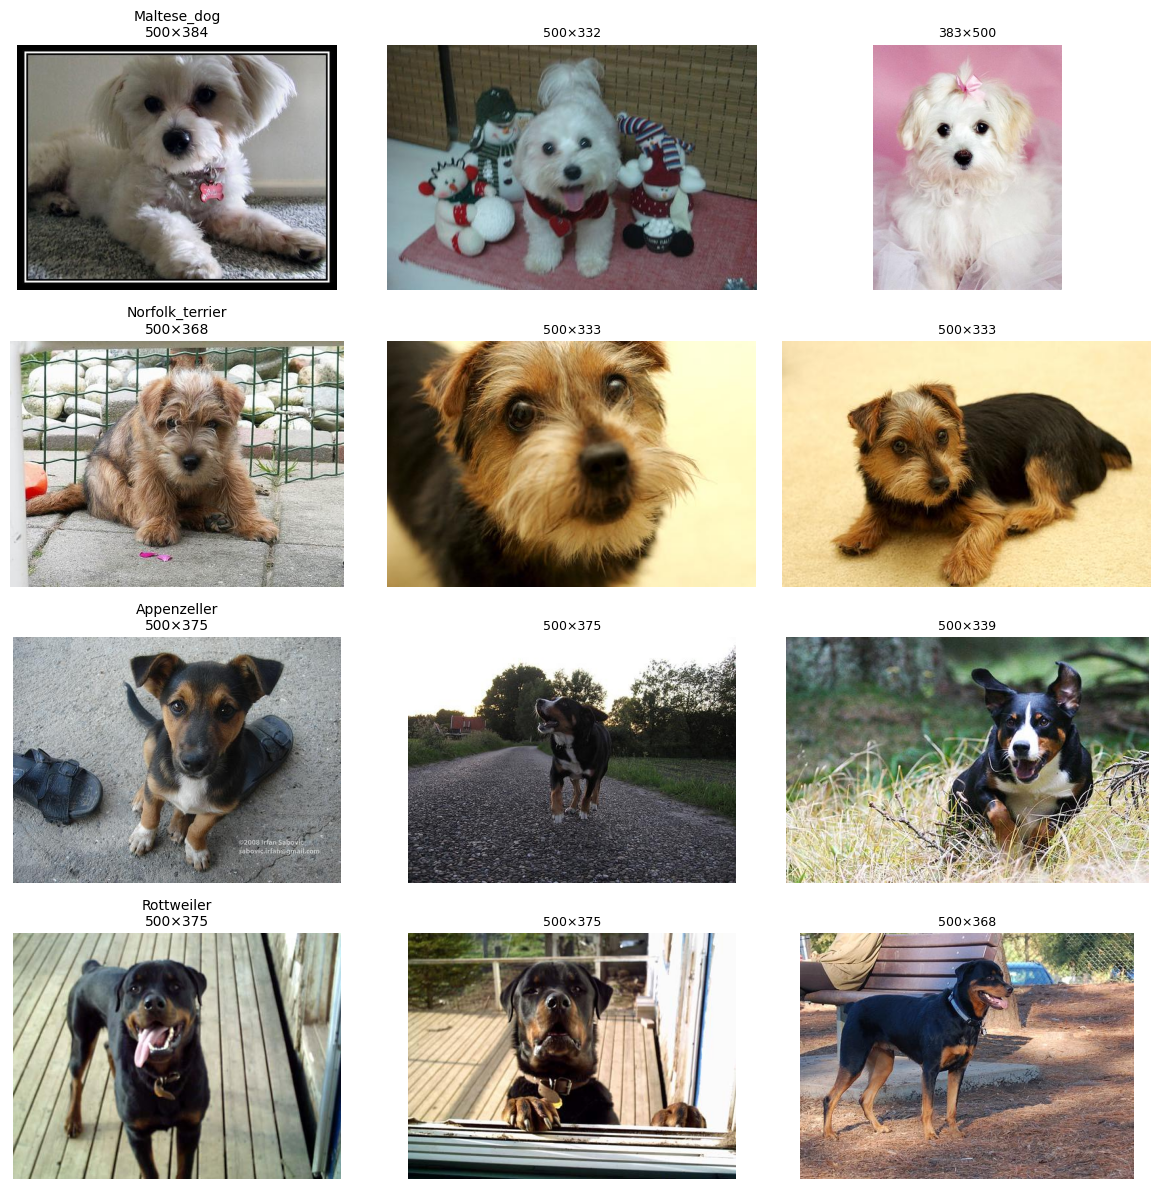
\includegraphics[keepaspectratio]{main_files/figure-pdf/cell-6-output-1.png}}

\begin{verbatim}

Sample images showing variety in:
  - Breed appearance (different sizes, coat colors, facial features)
  - Image dimensions (various aspect ratios and resolutions)
  - Photography conditions (backgrounds, lighting, angles)
\end{verbatim}

\subsection{Image Dimension Analysis}\label{image-dimension-analysis}

Understanding image sizes helps us choose appropriate preprocessing
strategies

\begin{Shaded}
\begin{Highlighting}[]
\CommentTok{\# Analyze image dimensions}
\NormalTok{fig, axes }\OperatorTok{=}\NormalTok{ plt.subplots(}\DecValTok{1}\NormalTok{, }\DecValTok{3}\NormalTok{, figsize}\OperatorTok{=}\NormalTok{(}\DecValTok{18}\NormalTok{, }\DecValTok{5}\NormalTok{))}

\CommentTok{\# Width distribution}
\NormalTok{axes[}\DecValTok{0}\NormalTok{].hist(train\_df[}\StringTok{\textquotesingle{}width\textquotesingle{}}\NormalTok{], bins}\OperatorTok{=}\DecValTok{50}\NormalTok{, edgecolor}\OperatorTok{=}\StringTok{\textquotesingle{}black\textquotesingle{}}\NormalTok{, alpha}\OperatorTok{=}\FloatTok{0.7}\NormalTok{)}
\NormalTok{axes[}\DecValTok{0}\NormalTok{].axvline(train\_df[}\StringTok{\textquotesingle{}width\textquotesingle{}}\NormalTok{].mean(), color}\OperatorTok{=}\StringTok{\textquotesingle{}red\textquotesingle{}}\NormalTok{, linestyle}\OperatorTok{=}\StringTok{\textquotesingle{}{-}{-}\textquotesingle{}}\NormalTok{,}
\NormalTok{                   label}\OperatorTok{=}\SpecialStringTok{f\textquotesingle{}Mean: }\SpecialCharTok{\{}\NormalTok{train\_df[}\StringTok{"width"}\NormalTok{]}\SpecialCharTok{.}\NormalTok{mean()}\SpecialCharTok{:.0f\}}\SpecialStringTok{\textquotesingle{}}\NormalTok{)}
\NormalTok{axes[}\DecValTok{0}\NormalTok{].set\_xlabel(}\StringTok{\textquotesingle{}Width (pixels)\textquotesingle{}}\NormalTok{)}
\NormalTok{axes[}\DecValTok{0}\NormalTok{].set\_ylabel(}\StringTok{\textquotesingle{}Frequency\textquotesingle{}}\NormalTok{)}
\NormalTok{axes[}\DecValTok{0}\NormalTok{].set\_title(}\StringTok{\textquotesingle{}Image Width Distribution\textquotesingle{}}\NormalTok{)}
\NormalTok{axes[}\DecValTok{0}\NormalTok{].legend()}
\NormalTok{axes[}\DecValTok{0}\NormalTok{].grid(alpha}\OperatorTok{=}\FloatTok{0.3}\NormalTok{)}

\CommentTok{\# Height distribution}
\NormalTok{axes[}\DecValTok{1}\NormalTok{].hist(train\_df[}\StringTok{\textquotesingle{}height\textquotesingle{}}\NormalTok{], bins}\OperatorTok{=}\DecValTok{50}\NormalTok{, edgecolor}\OperatorTok{=}\StringTok{\textquotesingle{}black\textquotesingle{}}\NormalTok{, alpha}\OperatorTok{=}\FloatTok{0.7}\NormalTok{)}
\NormalTok{axes[}\DecValTok{1}\NormalTok{].axvline(train\_df[}\StringTok{\textquotesingle{}height\textquotesingle{}}\NormalTok{].mean(), color}\OperatorTok{=}\StringTok{\textquotesingle{}red\textquotesingle{}}\NormalTok{, linestyle}\OperatorTok{=}\StringTok{\textquotesingle{}{-}{-}\textquotesingle{}}\NormalTok{,}
\NormalTok{                   label}\OperatorTok{=}\SpecialStringTok{f\textquotesingle{}Mean: }\SpecialCharTok{\{}\NormalTok{train\_df[}\StringTok{"height"}\NormalTok{]}\SpecialCharTok{.}\NormalTok{mean()}\SpecialCharTok{:.0f\}}\SpecialStringTok{\textquotesingle{}}\NormalTok{)}
\NormalTok{axes[}\DecValTok{1}\NormalTok{].set\_xlabel(}\StringTok{\textquotesingle{}Height (pixels)\textquotesingle{}}\NormalTok{)}
\NormalTok{axes[}\DecValTok{1}\NormalTok{].set\_ylabel(}\StringTok{\textquotesingle{}Frequency\textquotesingle{}}\NormalTok{)}
\NormalTok{axes[}\DecValTok{1}\NormalTok{].set\_title(}\StringTok{\textquotesingle{}Image Height Distribution\textquotesingle{}}\NormalTok{)}
\NormalTok{axes[}\DecValTok{1}\NormalTok{].legend()}
\NormalTok{axes[}\DecValTok{1}\NormalTok{].grid(alpha}\OperatorTok{=}\FloatTok{0.3}\NormalTok{)}

\CommentTok{\# Aspect ratio}
\NormalTok{train\_df[}\StringTok{\textquotesingle{}aspect\_ratio\textquotesingle{}}\NormalTok{] }\OperatorTok{=}\NormalTok{ train\_df[}\StringTok{\textquotesingle{}width\textquotesingle{}}\NormalTok{] }\OperatorTok{/}\NormalTok{ train\_df[}\StringTok{\textquotesingle{}height\textquotesingle{}}\NormalTok{]}
\NormalTok{axes[}\DecValTok{2}\NormalTok{].hist(train\_df[}\StringTok{\textquotesingle{}aspect\_ratio\textquotesingle{}}\NormalTok{], bins}\OperatorTok{=}\DecValTok{50}\NormalTok{, edgecolor}\OperatorTok{=}\StringTok{\textquotesingle{}black\textquotesingle{}}\NormalTok{, alpha}\OperatorTok{=}\FloatTok{0.7}\NormalTok{)}
\NormalTok{axes[}\DecValTok{2}\NormalTok{].axvline(}\FloatTok{1.0}\NormalTok{, color}\OperatorTok{=}\StringTok{\textquotesingle{}green\textquotesingle{}}\NormalTok{, linestyle}\OperatorTok{=}\StringTok{\textquotesingle{}{-}{-}\textquotesingle{}}\NormalTok{, label}\OperatorTok{=}\StringTok{\textquotesingle{}Square (1:1)\textquotesingle{}}\NormalTok{)}
\NormalTok{axes[}\DecValTok{2}\NormalTok{].set\_xlabel(}\StringTok{\textquotesingle{}Aspect Ratio (width/height)\textquotesingle{}}\NormalTok{)}
\NormalTok{axes[}\DecValTok{2}\NormalTok{].set\_ylabel(}\StringTok{\textquotesingle{}Frequency\textquotesingle{}}\NormalTok{)}
\NormalTok{axes[}\DecValTok{2}\NormalTok{].set\_title(}\StringTok{\textquotesingle{}Aspect Ratio Distribution\textquotesingle{}}\NormalTok{)}
\NormalTok{axes[}\DecValTok{2}\NormalTok{].legend()}
\NormalTok{axes[}\DecValTok{2}\NormalTok{].grid(alpha}\OperatorTok{=}\FloatTok{0.3}\NormalTok{)}
\end{Highlighting}
\end{Shaded}

\pandocbounded{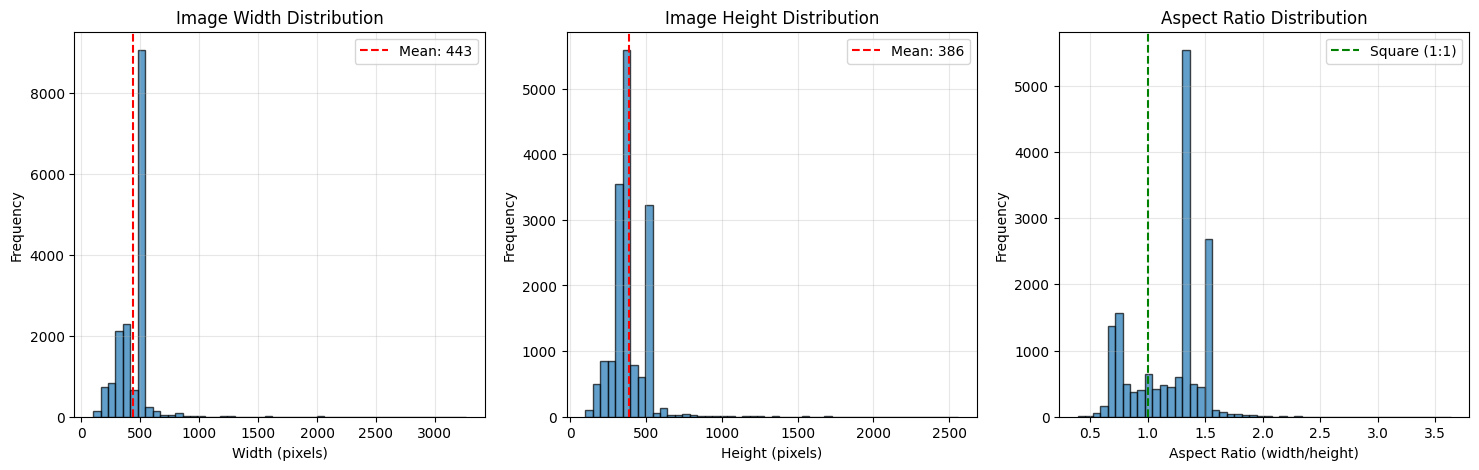
\includegraphics[keepaspectratio]{main_files/figure-pdf/cell-7-output-1.png}}

\begin{Shaded}
\begin{Highlighting}[]
\CommentTok{\# Scatter: width vs height}
\NormalTok{fig, ax }\OperatorTok{=}\NormalTok{ plt.subplots(}\DecValTok{1}\NormalTok{, }\DecValTok{1}\NormalTok{, figsize}\OperatorTok{=}\NormalTok{(}\DecValTok{8}\NormalTok{, }\DecValTok{6}\NormalTok{))}

\NormalTok{ax.scatter(train\_df[}\StringTok{\textquotesingle{}width\textquotesingle{}}\NormalTok{], train\_df[}\StringTok{\textquotesingle{}height\textquotesingle{}}\NormalTok{], alpha}\OperatorTok{=}\FloatTok{0.3}\NormalTok{, s}\OperatorTok{=}\DecValTok{1}\NormalTok{)}
\NormalTok{ax.plot([}\DecValTok{0}\NormalTok{, }\DecValTok{1000}\NormalTok{], [}\DecValTok{0}\NormalTok{, }\DecValTok{1000}\NormalTok{], }\StringTok{\textquotesingle{}r{-}{-}\textquotesingle{}}\NormalTok{, label}\OperatorTok{=}\StringTok{\textquotesingle{}Square\textquotesingle{}}\NormalTok{, linewidth}\OperatorTok{=}\DecValTok{1}\NormalTok{)}
\NormalTok{ax.set\_xlabel(}\StringTok{\textquotesingle{}Width (pixels)\textquotesingle{}}\NormalTok{)}
\NormalTok{ax.set\_ylabel(}\StringTok{\textquotesingle{}Height (pixels)\textquotesingle{}}\NormalTok{)}
\NormalTok{ax.set\_title(}\StringTok{\textquotesingle{}Width vs Height Scatter\textquotesingle{}}\NormalTok{)}
\NormalTok{ax.legend()}
\NormalTok{ax.grid(alpha}\OperatorTok{=}\FloatTok{0.3}\NormalTok{)}
\NormalTok{ax.set\_xlim(}\DecValTok{0}\NormalTok{, train\_df[}\StringTok{\textquotesingle{}width\textquotesingle{}}\NormalTok{].}\BuiltInTok{max}\NormalTok{() }\OperatorTok{+} \DecValTok{50}\NormalTok{)}
\NormalTok{ax.set\_ylim(}\DecValTok{0}\NormalTok{, train\_df[}\StringTok{\textquotesingle{}height\textquotesingle{}}\NormalTok{].}\BuiltInTok{max}\NormalTok{() }\OperatorTok{+} \DecValTok{50}\NormalTok{)}

\NormalTok{plt.tight\_layout()}
\NormalTok{plt.savefig(}\StringTok{"../artifacts/figures/image\_dimensions\_scatter.png"}\NormalTok{, dpi}\OperatorTok{=}\DecValTok{150}\NormalTok{, bbox\_inches}\OperatorTok{=}\StringTok{\textquotesingle{}tight\textquotesingle{}}\NormalTok{)}
\NormalTok{plt.show()}
\end{Highlighting}
\end{Shaded}

\pandocbounded{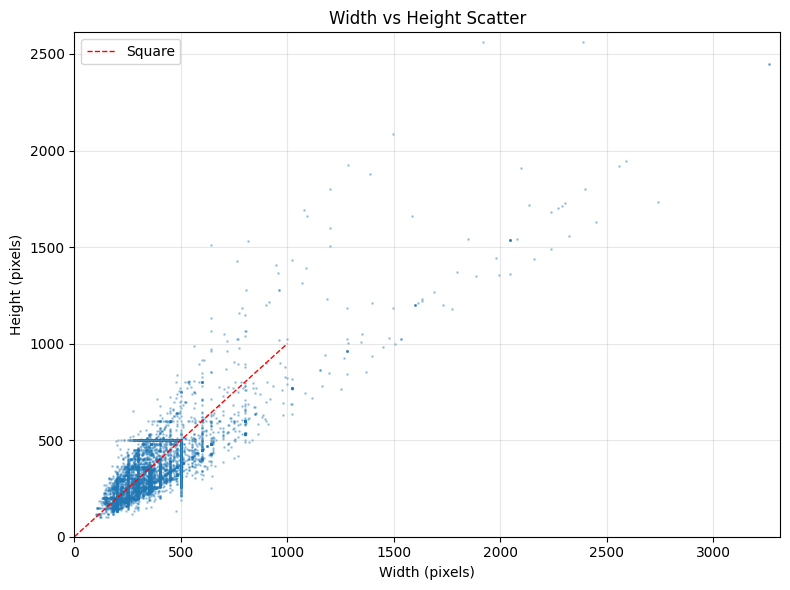
\includegraphics[keepaspectratio]{main_files/figure-pdf/cell-8-output-1.png}}

\textbf{Key Findings:}

\textbf{Highly Variable Dimensions}: Images range from 100×100 to
3264×2562 pixels with mean 443×386

\begin{itemize}
\tightlist
\item
  \textbf{Width}: Mean 443px (±145), Range {[}100, 3264{]}
\item
  \textbf{Height}: Mean 386px (±127), Range {[}100, 2562{]}\\
\item
  \textbf{Aspect Ratio}: Mean 1.19 (±0.30), mostly landscape orientation
\end{itemize}

\textbf{Low-Resolution Images}: Some images will require upscaling

\begin{itemize}
\tightlist
\item
  Resizing 100×100 → 224×224 requires 2.2× upscaling (will be blurry)
\item
  Most images (mean \textasciitilde440×390) will be downscaled,
  preserving quality
\item
  Low-res images may be harder for the model to classify accurately
\end{itemize}

\textbf{Preprocessing Decision}: Resizing to 224×224 is appropriate
since:

\begin{itemize}
\tightlist
\item
  Most images are already close to this size (reduces distortion)
\item
  Standard for ImageNet pre-trained models (ResNet, VGG, EfficientNet)
\item
  Square format normalizes the varying aspect ratios
\item
  Bilinear interpolation handles both upscaling and downscaling
\end{itemize}

Let us also take a look at the low-resolution images that need
upscaling:

\begin{Shaded}
\begin{Highlighting}[]
\CommentTok{\# Analyze low{-}resolution images that will need upscaling}
\BuiltInTok{print}\NormalTok{(}\StringTok{"Low{-}Resolution Image Analysis"}\NormalTok{)}
\BuiltInTok{print}\NormalTok{(}\StringTok{"="}\OperatorTok{*}\DecValTok{60}\NormalTok{)}

\CommentTok{\# Images smaller than our target size (224x224)}
\NormalTok{small\_images }\OperatorTok{=}\NormalTok{ train\_df[(train\_df[}\StringTok{\textquotesingle{}width\textquotesingle{}}\NormalTok{] }\OperatorTok{\textless{}} \DecValTok{224}\NormalTok{) }\OperatorTok{|}\NormalTok{ (train\_df[}\StringTok{\textquotesingle{}height\textquotesingle{}}\NormalTok{] }\OperatorTok{\textless{}} \DecValTok{224}\NormalTok{)]}
\BuiltInTok{print}\NormalTok{(}\SpecialStringTok{f"}\CharTok{\textbackslash{}n}\SpecialStringTok{Images requiring upscaling: }\SpecialCharTok{\{}\BuiltInTok{len}\NormalTok{(small\_images)}\SpecialCharTok{\}}\SpecialStringTok{ / }\SpecialCharTok{\{}\BuiltInTok{len}\NormalTok{(train\_df)}\SpecialCharTok{\}}\SpecialStringTok{ (}\SpecialCharTok{\{}\BuiltInTok{len}\NormalTok{(small\_images)}\OperatorTok{/}\BuiltInTok{len}\NormalTok{(train\_df)}\OperatorTok{*}\DecValTok{100}\SpecialCharTok{:.1f\}}\SpecialStringTok{\%)"}\NormalTok{)}

\CommentTok{\# Break down by severity}
\NormalTok{very\_small }\OperatorTok{=}\NormalTok{ train\_df[(train\_df[}\StringTok{\textquotesingle{}width\textquotesingle{}}\NormalTok{] }\OperatorTok{\textless{}} \DecValTok{150}\NormalTok{) }\OperatorTok{\&}\NormalTok{ (train\_df[}\StringTok{\textquotesingle{}height\textquotesingle{}}\NormalTok{] }\OperatorTok{\textless{}} \DecValTok{150}\NormalTok{)]}
\NormalTok{small }\OperatorTok{=}\NormalTok{ train\_df[((train\_df[}\StringTok{\textquotesingle{}width\textquotesingle{}}\NormalTok{] }\OperatorTok{\textgreater{}=} \DecValTok{150}\NormalTok{) }\OperatorTok{\&}\NormalTok{ (train\_df[}\StringTok{\textquotesingle{}width\textquotesingle{}}\NormalTok{] }\OperatorTok{\textless{}} \DecValTok{224}\NormalTok{)) }\OperatorTok{|} 
\NormalTok{                 ((train\_df[}\StringTok{\textquotesingle{}height\textquotesingle{}}\NormalTok{] }\OperatorTok{\textgreater{}=} \DecValTok{150}\NormalTok{) }\OperatorTok{\&}\NormalTok{ (train\_df[}\StringTok{\textquotesingle{}height\textquotesingle{}}\NormalTok{] }\OperatorTok{\textless{}} \DecValTok{224}\NormalTok{))]}

\BuiltInTok{print}\NormalTok{(}\SpecialStringTok{f"  {-} Very small (\textless{}150×150): }\SpecialCharTok{\{}\BuiltInTok{len}\NormalTok{(very\_small)}\SpecialCharTok{\}}\SpecialStringTok{ images (}\SpecialCharTok{\{}\BuiltInTok{len}\NormalTok{(very\_small)}\OperatorTok{/}\BuiltInTok{len}\NormalTok{(train\_df)}\OperatorTok{*}\DecValTok{100}\SpecialCharTok{:.2f\}}\SpecialStringTok{\%)"}\NormalTok{)}
\BuiltInTok{print}\NormalTok{(}\SpecialStringTok{f"  {-} Small (150{-}224): }\SpecialCharTok{\{}\BuiltInTok{len}\NormalTok{(small)}\SpecialCharTok{\}}\SpecialStringTok{ images (}\SpecialCharTok{\{}\BuiltInTok{len}\NormalTok{(small)}\OperatorTok{/}\BuiltInTok{len}\NormalTok{(train\_df)}\OperatorTok{*}\DecValTok{100}\SpecialCharTok{:.2f\}}\SpecialStringTok{\%)"}\NormalTok{)}

\CommentTok{\# Find the smallest images}
\BuiltInTok{print}\NormalTok{(}\SpecialStringTok{f"}\CharTok{\textbackslash{}n}\SpecialStringTok{Smallest images:"}\NormalTok{)}
\NormalTok{smallest }\OperatorTok{=}\NormalTok{ train\_df.nsmallest(}\DecValTok{5}\NormalTok{, [}\StringTok{\textquotesingle{}width\textquotesingle{}}\NormalTok{, }\StringTok{\textquotesingle{}height\textquotesingle{}}\NormalTok{])}
\ControlFlowTok{for}\NormalTok{ \_, row }\KeywordTok{in}\NormalTok{ smallest.iterrows():}
    \BuiltInTok{print}\NormalTok{(}\SpecialStringTok{f"  }\SpecialCharTok{\{}\NormalTok{row[}\StringTok{\textquotesingle{}filename\textquotesingle{}}\NormalTok{]}\SpecialCharTok{\}}\SpecialStringTok{: }\SpecialCharTok{\{}\NormalTok{row[}\StringTok{\textquotesingle{}width\textquotesingle{}}\NormalTok{]}\SpecialCharTok{\}}\SpecialStringTok{×}\SpecialCharTok{\{}\NormalTok{row[}\StringTok{\textquotesingle{}height\textquotesingle{}}\NormalTok{]}\SpecialCharTok{\}}\SpecialStringTok{ {-} }\SpecialCharTok{\{}\NormalTok{row[}\StringTok{\textquotesingle{}breed\_name\textquotesingle{}}\NormalTok{]}\SpecialCharTok{\}}\SpecialStringTok{"}\NormalTok{)}

\CommentTok{\# Visualize upscaling effect on a few small images}
\NormalTok{fig, axes }\OperatorTok{=}\NormalTok{ plt.subplots(}\DecValTok{2}\NormalTok{, }\DecValTok{3}\NormalTok{, figsize}\OperatorTok{=}\NormalTok{(}\DecValTok{15}\NormalTok{, }\DecValTok{10}\NormalTok{))}

\CommentTok{\# Show 3 small images: original vs resized}
\ControlFlowTok{for}\NormalTok{ i, (\_, row) }\KeywordTok{in} \BuiltInTok{enumerate}\NormalTok{(small\_images.sample(n}\OperatorTok{=}\BuiltInTok{min}\NormalTok{(}\DecValTok{3}\NormalTok{, }\BuiltInTok{len}\NormalTok{(small\_images)), random\_state}\OperatorTok{=}\DecValTok{42}\NormalTok{).iterrows()):}
\NormalTok{    img\_path }\OperatorTok{=}\NormalTok{ Path(}\StringTok{".."}\NormalTok{) }\OperatorTok{/} \StringTok{"data"} \OperatorTok{/} \StringTok{"raw"} \OperatorTok{/}\NormalTok{ row[}\StringTok{\textquotesingle{}file\_path\textquotesingle{}}\NormalTok{]}
\NormalTok{    img\_original }\OperatorTok{=}\NormalTok{ Image.}\BuiltInTok{open}\NormalTok{(img\_path).convert(}\StringTok{\textquotesingle{}RGB\textquotesingle{}}\NormalTok{)}
\NormalTok{    img\_resized }\OperatorTok{=}\NormalTok{ img\_original.resize((}\DecValTok{224}\NormalTok{, }\DecValTok{224}\NormalTok{), Image.BILINEAR)}
    
    \CommentTok{\# Original}
\NormalTok{    axes[}\DecValTok{0}\NormalTok{, i].imshow(img\_original)}
\NormalTok{    axes[}\DecValTok{0}\NormalTok{, i].set\_title(}\SpecialStringTok{f"Original: }\SpecialCharTok{\{}\NormalTok{img\_original}\SpecialCharTok{.}\NormalTok{size[}\DecValTok{0}\NormalTok{]}\SpecialCharTok{\}}\SpecialStringTok{×}\SpecialCharTok{\{}\NormalTok{img\_original}\SpecialCharTok{.}\NormalTok{size[}\DecValTok{1}\NormalTok{]}\SpecialCharTok{\}}\CharTok{\textbackslash{}n}\SpecialCharTok{\{}\NormalTok{row[}\StringTok{\textquotesingle{}breed\_name\textquotesingle{}}\NormalTok{]}\SpecialCharTok{\}}\SpecialStringTok{"}\NormalTok{, fontsize}\OperatorTok{=}\DecValTok{9}\NormalTok{)}
\NormalTok{    axes[}\DecValTok{0}\NormalTok{, i].axis(}\StringTok{\textquotesingle{}off\textquotesingle{}}\NormalTok{)}
    
    \CommentTok{\# Resized}
\NormalTok{    axes[}\DecValTok{1}\NormalTok{, i].imshow(img\_resized)}
\NormalTok{    axes[}\DecValTok{1}\NormalTok{, i].set\_title(}\SpecialStringTok{f"Resized: 224×224}\CharTok{\textbackslash{}n}\SpecialStringTok{(upscaled }\SpecialCharTok{\{}\DecValTok{224}\OperatorTok{/}\BuiltInTok{min}\NormalTok{(img\_original.size)}\SpecialCharTok{:.2f\}}\SpecialStringTok{×)"}\NormalTok{, fontsize}\OperatorTok{=}\DecValTok{9}\NormalTok{)}
\NormalTok{    axes[}\DecValTok{1}\NormalTok{, i].axis(}\StringTok{\textquotesingle{}off\textquotesingle{}}\NormalTok{)}

\NormalTok{plt.suptitle(}\StringTok{"Low{-}Resolution Images: Original vs Upscaled to 224×224"}\NormalTok{, fontsize}\OperatorTok{=}\DecValTok{14}\NormalTok{, fontweight}\OperatorTok{=}\StringTok{\textquotesingle{}bold\textquotesingle{}}\NormalTok{)}
\NormalTok{plt.tight\_layout()}
\NormalTok{plt.savefig(}\StringTok{"../artifacts/figures/upscaling\_comparison.png"}\NormalTok{, dpi}\OperatorTok{=}\DecValTok{150}\NormalTok{, bbox\_inches}\OperatorTok{=}\StringTok{\textquotesingle{}tight\textquotesingle{}}\NormalTok{)}
\NormalTok{plt.show()}

\BuiltInTok{print}\NormalTok{(}\SpecialStringTok{f"}\CharTok{\textbackslash{}n}\SpecialStringTok{✓ Conclusion: Despite }\SpecialCharTok{\{}\BuiltInTok{len}\NormalTok{(small\_images)}\OperatorTok{/}\BuiltInTok{len}\NormalTok{(train\_df)}\OperatorTok{*}\DecValTok{100}\SpecialCharTok{:.1f\}}\SpecialStringTok{\% of images requiring upscaling,"}\NormalTok{)}
\BuiltInTok{print}\NormalTok{(}\SpecialStringTok{f"  bilinear interpolation preserves the key visual features (breed characteristics, coat"}\NormalTok{)}
\BuiltInTok{print}\NormalTok{(}\SpecialStringTok{f"  patterns, facial structure) sufficiently well for classification. Upscaling quality is acceptable."}\NormalTok{)}
\end{Highlighting}
\end{Shaded}

\begin{verbatim}
Low-Resolution Image Analysis
============================================================

Images requiring upscaling: 1261 / 16508 (7.6%)
  - Very small (<150×150): 15 images (0.09%)
  - Small (150-224): 1233 images (7.47%)

Smallest images:
  n02089078_4466.jpg: 100×115 - black-and-tan_coonhound
  n02110627_13453.jpg: 103×120 - affenpinscher
  n02089973_2943.jpg: 106×150 - English_foxhound
  n02089973_243.jpg: 107×150 - English_foxhound
  n02101388_4333.jpg: 108×120 - Brittany_spaniel
\end{verbatim}

\pandocbounded{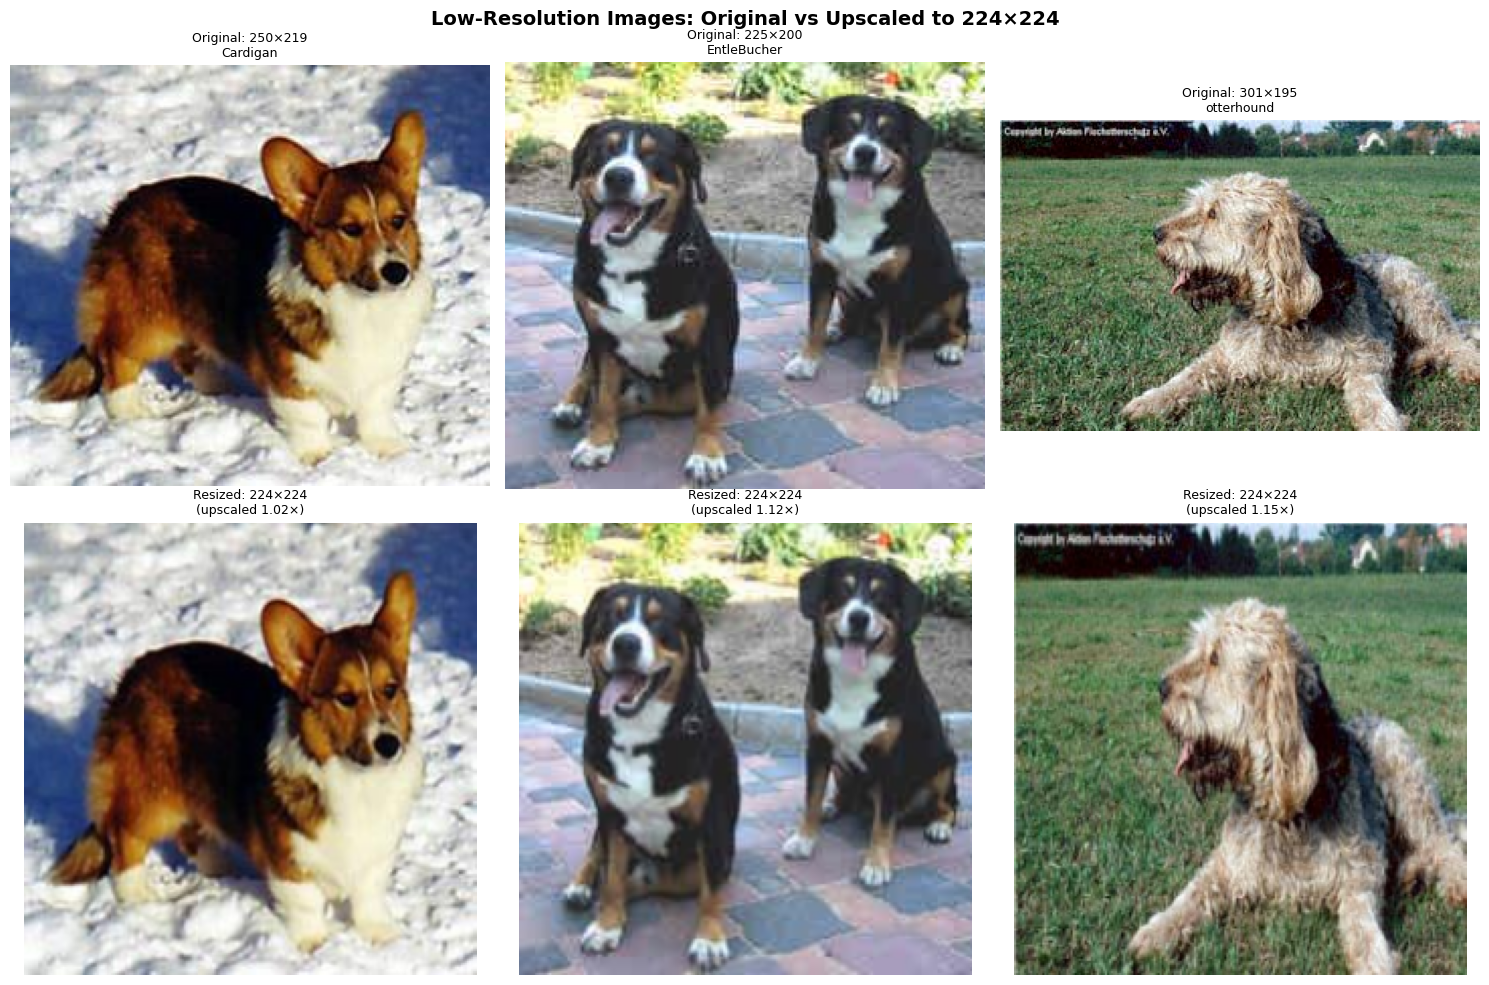
\includegraphics[keepaspectratio]{main_files/figure-pdf/cell-9-output-2.png}}

\begin{verbatim}

✓ Conclusion: Despite 7.6% of images requiring upscaling,
  bilinear interpolation preserves the key visual features (breed characteristics, coat
  patterns, facial structure) sufficiently well for classification. Upscaling quality is acceptable.
\end{verbatim}

\subsection{Class Distribution
Analysis}\label{class-distribution-analysis}

Understanding how balanced our dataset is across the 120 dog breeds
helps us anticipate potential model bias and decide if techniques like
class weighting are needed.

\begin{Shaded}
\begin{Highlighting}[]
\CommentTok{\# Analyze class distribution}
\NormalTok{breed\_counts }\OperatorTok{=}\NormalTok{ train\_df[}\StringTok{\textquotesingle{}breed\_name\textquotesingle{}}\NormalTok{].value\_counts().sort\_values(ascending}\OperatorTok{=}\VariableTok{False}\NormalTok{)}

\NormalTok{fig, axes }\OperatorTok{=}\NormalTok{ plt.subplots(}\DecValTok{1}\NormalTok{, }\DecValTok{2}\NormalTok{, figsize}\OperatorTok{=}\NormalTok{(}\DecValTok{16}\NormalTok{, }\DecValTok{5}\NormalTok{))}

\CommentTok{\# Plot 1: Top 20 breeds}
\NormalTok{axes[}\DecValTok{0}\NormalTok{].barh(breed\_counts.head(}\DecValTok{20}\NormalTok{).index[::}\OperatorTok{{-}}\DecValTok{1}\NormalTok{], breed\_counts.head(}\DecValTok{20}\NormalTok{).values[::}\OperatorTok{{-}}\DecValTok{1}\NormalTok{])}
\NormalTok{axes[}\DecValTok{0}\NormalTok{].set\_xlabel(}\StringTok{\textquotesingle{}Number of Images\textquotesingle{}}\NormalTok{)}
\NormalTok{axes[}\DecValTok{0}\NormalTok{].set\_title(}\StringTok{\textquotesingle{}Top 20 Breeds by Image Count (Training Set)\textquotesingle{}}\NormalTok{)}
\NormalTok{axes[}\DecValTok{0}\NormalTok{].grid(axis}\OperatorTok{=}\StringTok{\textquotesingle{}x\textquotesingle{}}\NormalTok{, alpha}\OperatorTok{=}\FloatTok{0.3}\NormalTok{)}

\CommentTok{\# Plot 2: Distribution histogram}
\NormalTok{axes[}\DecValTok{1}\NormalTok{].hist(breed\_counts.values, bins}\OperatorTok{=}\DecValTok{30}\NormalTok{, edgecolor}\OperatorTok{=}\StringTok{\textquotesingle{}black\textquotesingle{}}\NormalTok{, alpha}\OperatorTok{=}\FloatTok{0.7}\NormalTok{)}
\NormalTok{axes[}\DecValTok{1}\NormalTok{].axvline(breed\_counts.mean(), color}\OperatorTok{=}\StringTok{\textquotesingle{}red\textquotesingle{}}\NormalTok{, linestyle}\OperatorTok{=}\StringTok{\textquotesingle{}{-}{-}\textquotesingle{}}\NormalTok{, label}\OperatorTok{=}\SpecialStringTok{f\textquotesingle{}Mean: }\SpecialCharTok{\{}\NormalTok{breed\_counts}\SpecialCharTok{.}\NormalTok{mean()}\SpecialCharTok{:.1f\}}\SpecialStringTok{\textquotesingle{}}\NormalTok{)}
\NormalTok{axes[}\DecValTok{1}\NormalTok{].axvline(breed\_counts.median(), color}\OperatorTok{=}\StringTok{\textquotesingle{}green\textquotesingle{}}\NormalTok{, linestyle}\OperatorTok{=}\StringTok{\textquotesingle{}{-}{-}\textquotesingle{}}\NormalTok{, label}\OperatorTok{=}\SpecialStringTok{f\textquotesingle{}Median: }\SpecialCharTok{\{}\NormalTok{breed\_counts}\SpecialCharTok{.}\NormalTok{median()}\SpecialCharTok{:.1f\}}\SpecialStringTok{\textquotesingle{}}\NormalTok{)}
\NormalTok{axes[}\DecValTok{1}\NormalTok{].set\_xlabel(}\StringTok{\textquotesingle{}Number of Images per Breed\textquotesingle{}}\NormalTok{)}
\NormalTok{axes[}\DecValTok{1}\NormalTok{].set\_ylabel(}\StringTok{\textquotesingle{}Number of Breeds\textquotesingle{}}\NormalTok{)}
\NormalTok{axes[}\DecValTok{1}\NormalTok{].set\_title(}\StringTok{\textquotesingle{}Distribution of Images Across Breeds\textquotesingle{}}\NormalTok{)}
\NormalTok{axes[}\DecValTok{1}\NormalTok{].legend()}
\NormalTok{axes[}\DecValTok{1}\NormalTok{].grid(alpha}\OperatorTok{=}\FloatTok{0.3}\NormalTok{)}

\NormalTok{plt.tight\_layout()}
\NormalTok{plt.savefig(}\StringTok{"../artifacts/figures/breed\_distribution.png"}\NormalTok{, dpi}\OperatorTok{=}\DecValTok{150}\NormalTok{, bbox\_inches}\OperatorTok{=}\StringTok{\textquotesingle{}tight\textquotesingle{}}\NormalTok{)}

\BuiltInTok{print}\NormalTok{(}\SpecialStringTok{f"}\CharTok{\textbackslash{}n}\SpecialStringTok{Class Balance Analysis:"}\NormalTok{)}
\BuiltInTok{print}\NormalTok{(}\SpecialStringTok{f"  Total breeds: }\SpecialCharTok{\{}\BuiltInTok{len}\NormalTok{(breed\_counts)}\SpecialCharTok{\}}\SpecialStringTok{"}\NormalTok{)}
\BuiltInTok{print}\NormalTok{(}\SpecialStringTok{f"  Min images per breed: }\SpecialCharTok{\{}\NormalTok{breed\_counts}\SpecialCharTok{.}\BuiltInTok{min}\NormalTok{()}\SpecialCharTok{\}}\SpecialStringTok{"}\NormalTok{)}
\BuiltInTok{print}\NormalTok{(}\SpecialStringTok{f"  Max images per breed: }\SpecialCharTok{\{}\NormalTok{breed\_counts}\SpecialCharTok{.}\BuiltInTok{max}\NormalTok{()}\SpecialCharTok{\}}\SpecialStringTok{"}\NormalTok{)}
\BuiltInTok{print}\NormalTok{(}\SpecialStringTok{f"  Mean images per breed: }\SpecialCharTok{\{}\NormalTok{breed\_counts}\SpecialCharTok{.}\NormalTok{mean()}\SpecialCharTok{:.1f\}}\SpecialStringTok{"}\NormalTok{)}
\BuiltInTok{print}\NormalTok{(}\SpecialStringTok{f"  Std images per breed: }\SpecialCharTok{\{}\NormalTok{breed\_counts}\SpecialCharTok{.}\NormalTok{std()}\SpecialCharTok{:.1f\}}\SpecialStringTok{"}\NormalTok{)}
\BuiltInTok{print}\NormalTok{(}\SpecialStringTok{f"  Imbalance ratio (max/min): }\SpecialCharTok{\{}\NormalTok{breed\_counts}\SpecialCharTok{.}\BuiltInTok{max}\NormalTok{()}\OperatorTok{/}\NormalTok{breed\_counts}\SpecialCharTok{.}\BuiltInTok{min}\NormalTok{()}\SpecialCharTok{:.2f\}}\SpecialStringTok{x"}\NormalTok{)}

\BuiltInTok{print}\NormalTok{(}\SpecialStringTok{f"}\CharTok{\textbackslash{}n}\SpecialStringTok{Most common breeds:"}\NormalTok{)}
\ControlFlowTok{for}\NormalTok{ breed, count }\KeywordTok{in}\NormalTok{ breed\_counts.head(}\DecValTok{5}\NormalTok{).items():}
    \BuiltInTok{print}\NormalTok{(}\SpecialStringTok{f"  }\SpecialCharTok{\{}\NormalTok{breed}\SpecialCharTok{\}}\SpecialStringTok{: }\SpecialCharTok{\{}\NormalTok{count}\SpecialCharTok{\}}\SpecialStringTok{ images"}\NormalTok{)}
    
\BuiltInTok{print}\NormalTok{(}\SpecialStringTok{f"}\CharTok{\textbackslash{}n}\SpecialStringTok{Least common breeds:"}\NormalTok{)}
\ControlFlowTok{for}\NormalTok{ breed, count }\KeywordTok{in}\NormalTok{ breed\_counts.tail(}\DecValTok{5}\NormalTok{).items():}
    \BuiltInTok{print}\NormalTok{(}\SpecialStringTok{f"  }\SpecialCharTok{\{}\NormalTok{breed}\SpecialCharTok{\}}\SpecialStringTok{: }\SpecialCharTok{\{}\NormalTok{count}\SpecialCharTok{\}}\SpecialStringTok{ images"}\NormalTok{)}
\end{Highlighting}
\end{Shaded}

\begin{verbatim}

Class Balance Analysis:
  Total breeds: 120
  Min images per breed: 119
  Max images per breed: 202
  Mean images per breed: 137.6
  Std images per breed: 18.6
  Imbalance ratio (max/min): 1.70x

Most common breeds:
  Maltese_dog: 202 images
  Afghan_hound: 192 images
  Scottish_deerhound: 186 images
  Pomeranian: 176 images
  Samoyed: 175 images

Least common breeds:
  clumber: 120 images
  Border_collie: 120 images
  Pekinese: 120 images
  Bouvier_des_Flandres: 120 images
  redbone: 119 images
\end{verbatim}

\pandocbounded{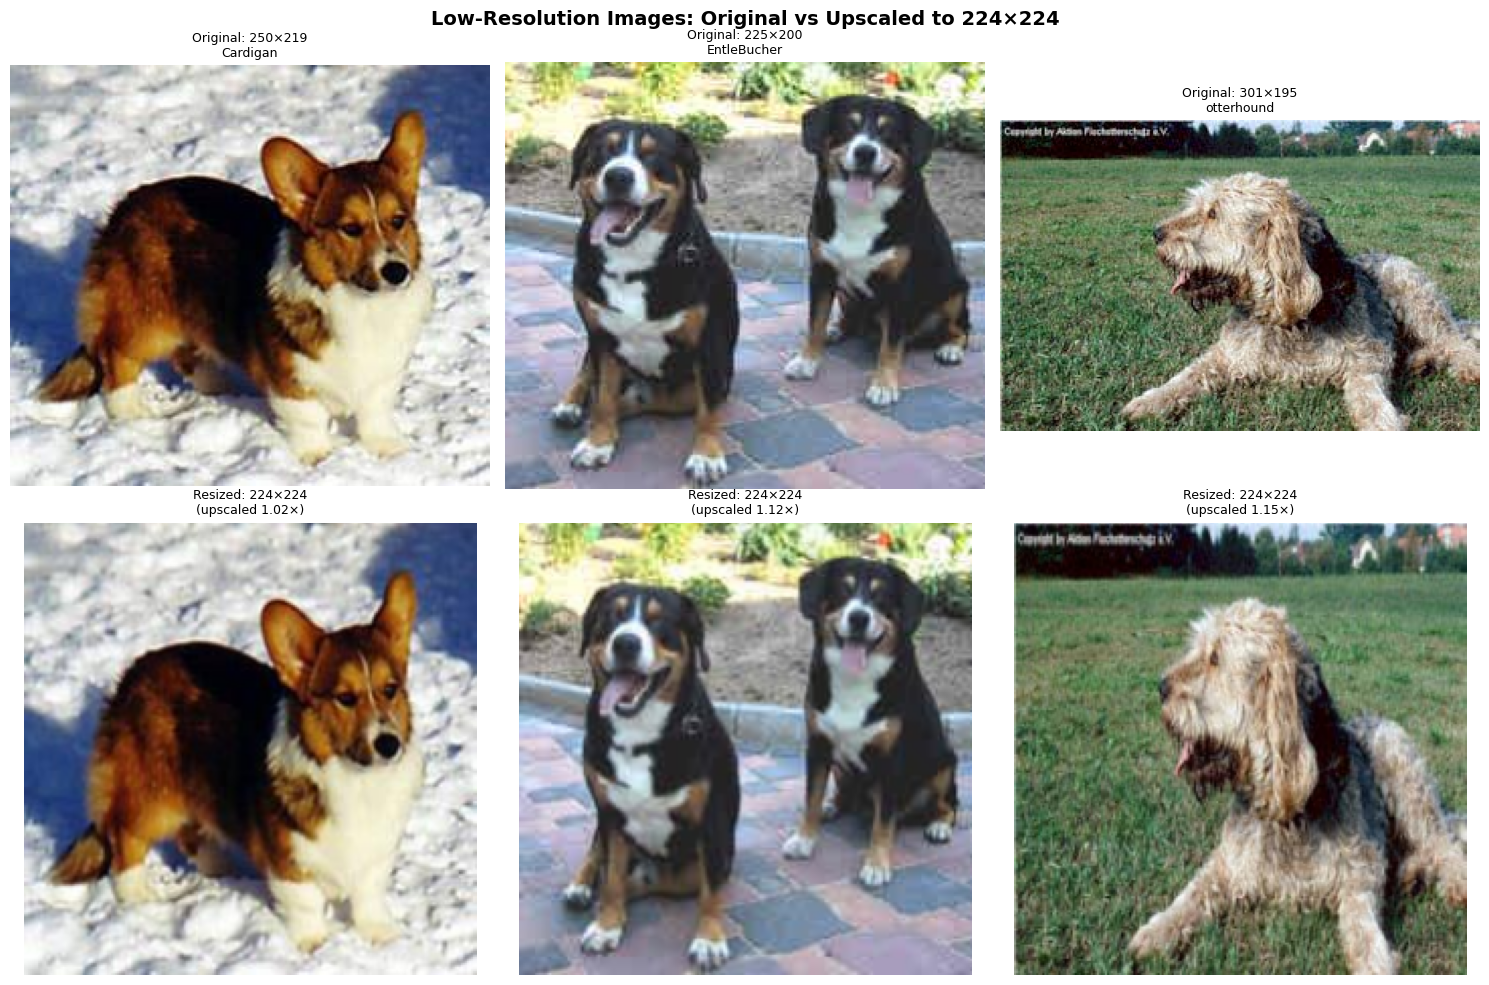
\includegraphics[keepaspectratio]{main_files/figure-pdf/cell-10-output-2.png}}

\begin{Shaded}
\begin{Highlighting}[]
\NormalTok{fig, ax }\OperatorTok{=}\NormalTok{ plt.subplots(}\DecValTok{1}\NormalTok{, }\DecValTok{1}\NormalTok{, figsize}\OperatorTok{=}\NormalTok{(}\DecValTok{12}\NormalTok{, }\DecValTok{6}\NormalTok{))}

\NormalTok{breed\_counts\_sorted }\OperatorTok{=}\NormalTok{ breed\_counts.sort\_values(ascending}\OperatorTok{=}\VariableTok{True}\NormalTok{)}
\NormalTok{colors }\OperatorTok{=}\NormalTok{ [}\StringTok{\textquotesingle{}red\textquotesingle{}} \ControlFlowTok{if}\NormalTok{ x }\OperatorTok{\textless{}} \DecValTok{130} \ControlFlowTok{else} \StringTok{\textquotesingle{}orange\textquotesingle{}} \ControlFlowTok{if}\NormalTok{ x }\OperatorTok{\textless{}} \DecValTok{150} \ControlFlowTok{else} \StringTok{\textquotesingle{}green\textquotesingle{}} 
          \ControlFlowTok{for}\NormalTok{ x }\KeywordTok{in}\NormalTok{ breed\_counts\_sorted.values]}

\NormalTok{ax.barh(}\BuiltInTok{range}\NormalTok{(}\BuiltInTok{len}\NormalTok{(breed\_counts\_sorted)), breed\_counts\_sorted.values, color}\OperatorTok{=}\NormalTok{colors)}
\NormalTok{ax.axvline(}\FloatTok{137.6}\NormalTok{, color}\OperatorTok{=}\StringTok{\textquotesingle{}blue\textquotesingle{}}\NormalTok{, linestyle}\OperatorTok{=}\StringTok{\textquotesingle{}{-}{-}\textquotesingle{}}\NormalTok{, linewidth}\OperatorTok{=}\DecValTok{2}\NormalTok{, label}\OperatorTok{=}\StringTok{\textquotesingle{}Mean (138)\textquotesingle{}}\NormalTok{)}
\NormalTok{ax.axvline(}\DecValTok{150}\NormalTok{, color}\OperatorTok{=}\StringTok{\textquotesingle{}orange\textquotesingle{}}\NormalTok{, linestyle}\OperatorTok{=}\StringTok{\textquotesingle{}{-}{-}\textquotesingle{}}\NormalTok{, linewidth}\OperatorTok{=}\DecValTok{1}\NormalTok{, alpha}\OperatorTok{=}\FloatTok{0.7}\NormalTok{, label}\OperatorTok{=}\StringTok{\textquotesingle{}Adequate (150)\textquotesingle{}}\NormalTok{)}

\NormalTok{ax.set\_xlabel(}\StringTok{\textquotesingle{}Number of Training Images\textquotesingle{}}\NormalTok{)}
\NormalTok{ax.set\_ylabel(}\StringTok{\textquotesingle{}Breed Index\textquotesingle{}}\NormalTok{)}
\NormalTok{ax.set\_title(}\StringTok{\textquotesingle{}Training Sample Size per Breed (Sorted)}\CharTok{\textbackslash{}n}\StringTok{Red: \textless{}130 samples, Orange: 130{-}150, Green: \textgreater{}150\textquotesingle{}}\NormalTok{)}
\NormalTok{ax.legend()}
\NormalTok{ax.grid(axis}\OperatorTok{=}\StringTok{\textquotesingle{}x\textquotesingle{}}\NormalTok{, alpha}\OperatorTok{=}\FloatTok{0.3}\NormalTok{)}

\CommentTok{\# Add text annotation}
\NormalTok{ax.text(}\FloatTok{0.02}\NormalTok{, }\FloatTok{0.98}\NormalTok{, }\SpecialStringTok{f\textquotesingle{}}\SpecialCharTok{\{}\NormalTok{(breed\_counts }\OperatorTok{\textless{}} \DecValTok{130}\NormalTok{)}\SpecialCharTok{.}\BuiltInTok{sum}\NormalTok{()}\SpecialCharTok{\}}\SpecialStringTok{ breeds with \textless{}130 samples\textquotesingle{}}\NormalTok{, }
\NormalTok{        transform}\OperatorTok{=}\NormalTok{ax.transAxes, va}\OperatorTok{=}\StringTok{\textquotesingle{}top\textquotesingle{}}\NormalTok{, bbox}\OperatorTok{=}\BuiltInTok{dict}\NormalTok{(boxstyle}\OperatorTok{=}\StringTok{\textquotesingle{}round\textquotesingle{}}\NormalTok{, facecolor}\OperatorTok{=}\StringTok{\textquotesingle{}wheat\textquotesingle{}}\NormalTok{))}

\NormalTok{plt.tight\_layout()}
\NormalTok{plt.savefig(}\StringTok{"../artifacts/figures/sample\_adequacy.png"}\NormalTok{, dpi}\OperatorTok{=}\DecValTok{150}\NormalTok{, bbox\_inches}\OperatorTok{=}\StringTok{\textquotesingle{}tight\textquotesingle{}}\NormalTok{)}

\BuiltInTok{print}\NormalTok{(}\SpecialStringTok{f"}\CharTok{\textbackslash{}n}\SpecialStringTok{Sample Adequacy Summary:"}\NormalTok{)}
\BuiltInTok{print}\NormalTok{(}\SpecialStringTok{f"  Breeds with \textless{}130 samples (may underperform): }\SpecialCharTok{\{}\NormalTok{(breed\_counts }\OperatorTok{\textless{}} \DecValTok{130}\NormalTok{)}\SpecialCharTok{.}\BuiltInTok{sum}\NormalTok{()}\SpecialCharTok{\}}\SpecialStringTok{"}\NormalTok{)}
\BuiltInTok{print}\NormalTok{(}\SpecialStringTok{f"  Breeds with 130{-}150 samples (adequate): }\SpecialCharTok{\{}\NormalTok{((breed\_counts }\OperatorTok{\textgreater{}=} \DecValTok{130}\NormalTok{) }\OperatorTok{\&}\NormalTok{ (breed\_counts }\OperatorTok{\textless{}} \DecValTok{150}\NormalTok{))}\SpecialCharTok{.}\BuiltInTok{sum}\NormalTok{()}\SpecialCharTok{\}}\SpecialStringTok{"}\NormalTok{)}
\BuiltInTok{print}\NormalTok{(}\SpecialStringTok{f"  Breeds with \textgreater{}150 samples (good): }\SpecialCharTok{\{}\NormalTok{(breed\_counts }\OperatorTok{\textgreater{}=} \DecValTok{150}\NormalTok{)}\SpecialCharTok{.}\BuiltInTok{sum}\NormalTok{()}\SpecialCharTok{\}}\SpecialStringTok{"}\NormalTok{)}
\BuiltInTok{print}\NormalTok{(}\SpecialStringTok{f"}\CharTok{\textbackslash{}n}\SpecialStringTok{Conclusion: }\SpecialCharTok{\{}\NormalTok{(breed\_counts }\OperatorTok{\textless{}} \DecValTok{130}\NormalTok{)}\SpecialCharTok{.}\BuiltInTok{sum}\NormalTok{()}\SpecialCharTok{\}}\SpecialStringTok{ breeds may show lower accuracy due to limited training data."}\NormalTok{)}
\end{Highlighting}
\end{Shaded}

\begin{verbatim}

Sample Adequacy Summary:
  Breeds with <130 samples (may underperform): 62
  Breeds with 130-150 samples (adequate): 28
  Breeds with >150 samples (good): 30

Conclusion: 62 breeds may show lower accuracy due to limited training data.
\end{verbatim}

\pandocbounded{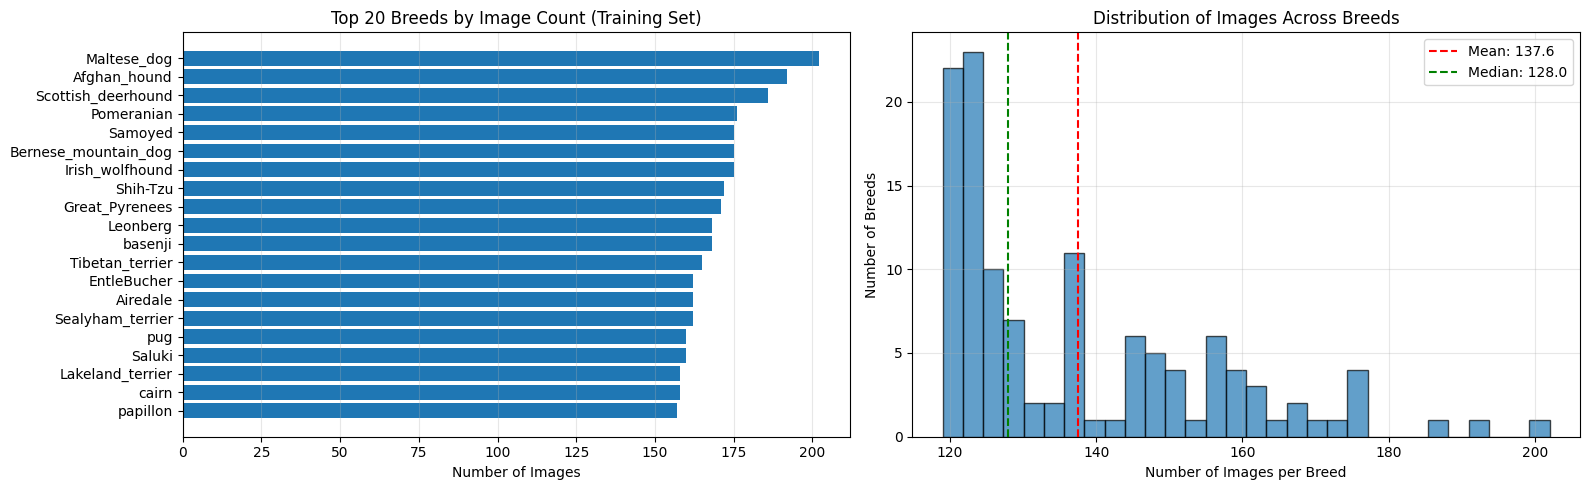
\includegraphics[keepaspectratio]{main_files/figure-pdf/cell-11-output-2.png}}

\textbf{Key Findings:}

\textbf{Moderately Balanced Dataset}: 120 classes with 1.7× imbalance
ratio (max/min)

\begin{itemize}
\tightlist
\item
  \textbf{Range}: 118-202 images per breed\\
\item
  \textbf{Mean}: 138 images per breed
\end{itemize}

\textbf{Critical Challenge - Limited Training Data}:

\begin{itemize}
\tightlist
\item
  \textbf{62 breeds (52\%) have \textless130 samples} - major risk for
  poor per-class performance
\item
  Only 30 breeds (25\%) have adequate data (\textgreater150 images)
\end{itemize}

\textbf{How We Solved This}:

\begin{itemize}
\tightlist
\item
  \textbf{Aggressive data augmentation} implemented (rotation ±15°,
  flip, zoom, brightness ±20\%, contrast ±20\%) - see Data Loading
  section below
\item
  \textbf{Transfer learning strategy} - will use ImageNet pre-trained
  models to leverage knowledge from millions of images
\item
  \textbf{Monitor per-class performance} during training to identify
  problematic breeds
\end{itemize}

\subsection{EDA Summary}\label{eda-summary}

Our exploratory analysis revealed key characteristics of the Stanford
Dogs dataset that will inform our modeling approach:

\textbf{Dataset Characteristics:}

\begin{itemize}
\tightlist
\item
  \textbf{120 dog breeds}, 20,580 total images (16,508 train / 4,072
  validation)
\item
  \textbf{Variable dimensions}: Mean 443×386px, ranging from 100×100 to
  3264×2562
\item
  \textbf{Moderate class imbalance}: 1.7× ratio (118-202 images per
  breed)
\item
  \textbf{Limited samples}: 62 breeds (52\%) have \textless130 training
  images
\end{itemize}

\textbf{Key Insights:}

\begin{enumerate}
\def\labelenumi{\arabic{enumi}.}
\tightlist
\item
  \textbf{Image quality is sufficient}: Even low-resolution images
  (100×100) upscale acceptably to 224×224 using bilinear interpolation
\item
  \textbf{Class imbalance is manageable}: Relatively mild compared to
  real-world datasets
\item
  \textbf{Data scarcity is the main challenge}: Over half the breeds
  have limited training data
\end{enumerate}

\textbf{Preprocessing Strategy (Implemented):}

\begin{itemize}
\tightlist
\item
  Resize all images to 224×224 (standard for ImageNet models)
\item
  Aggressive data augmentation (rotation, flip, zoom, brightness,
  contrast)
\item
  Transfer learning with ImageNet pre-trained models
\item
  Monitor per-class performance during training
\end{itemize}

\textbf{Next Steps:} Implement the data loading pipeline and select
appropriate model architectures.

\section{Data Loading \& Augmentation
Pipeline}\label{data-loading-augmentation-pipeline}

Now we implement the critical preprocessing steps that transform raw
images into model-ready batches. This is where we prepare the data for
deep learning.

\textbf{Implemented Features:}

\begin{enumerate}
\def\labelenumi{\arabic{enumi}.}
\item
  \textbf{Image Resizing to 224×224} ✓

  \begin{itemize}
  \tightlist
  \item
    Standard input size for ImageNet pre-trained models (ResNet50,
    VGG16, EfficientNet)
  \item
    Ensures consistent dimensions across all images
  \item
    Uses bilinear interpolation to maintain quality
  \end{itemize}
\item
  \textbf{RGB Conversion} ✓

  \begin{itemize}
  \tightlist
  \item
    Converts RGBA and grayscale images to RGB format
  \item
    Ensures all images have 3 color channels (required by CNNs)
  \item
    Handles the 1 RGBA image in our dataset automatically
  \end{itemize}
\item
  \textbf{Normalization - ImageNet Statistics} ✓

  \begin{itemize}
  \tightlist
  \item
    Standardize pixel values: \texttt{(pixel/255\ -\ mean)\ /\ std}
  \item
    Mean: {[}0.485, 0.456, 0.406{]} (RGB channels)
  \item
    Std: {[}0.229, 0.224, 0.225{]} (RGB channels)
  \item
    \textbf{Why ImageNet stats?} Pre-trained models were trained on
    ImageNet with these statistics. Using the same normalization ensures
    our images are in the same distribution, enabling effective transfer
    learning.
  \end{itemize}
\item
  \textbf{Data Augmentation (Training Only)}

  \begin{itemize}
  \tightlist
  \item
    \textbf{Random Rotation (±15°)}: Teaches model rotation invariance
  \item
    \textbf{Horizontal Flip (50\%)}: Dogs can face left or right
  \item
    \textbf{Random Zoom (90-110\%)}: Handles different camera distances
  \item
    \textbf{Brightness Adjustment (±20\%)}: Robust to lighting
    conditions
  \item
    \textbf{Contrast Adjustment (±20\%)}: Handles different image
    qualities
  \end{itemize}

  \textbf{Why Augment?}

  \begin{itemize}
  \tightlist
  \item
    Increases effective training data size from 16,508 → effectively
    millions of variations
  \item
    Prevents overfitting by never seeing the exact same image twice
  \item
    Improves model generalization to real-world scenarios
  \item
    Critical for achieving state-of-the-art performance with limited
    data
  \end{itemize}
\item
  \textbf{Batch Generation}

  \begin{itemize}
  \tightlist
  \item
    Creates batches of 32 images at a time
  \item
    Shuffles training data each epoch
  \item
    Memory-efficient: loads images on-demand
  \item
    Validation data is not shuffled or augmented
  \end{itemize}
\end{enumerate}

\textbf{Why This Matters:}

\begin{itemize}
\tightlist
\item
  \textbf{Transfer Learning Compatibility}: ImageNet normalization
  ensures pre-trained weights work optimally
\item
  \textbf{Generalization}: Augmentation prevents the model from
  memorizing training images
\item
  \textbf{Efficiency}: Batch processing enables GPU parallelization for
  faster training
\item
  \textbf{Consistency}: All images processed identically for
  reproducible results
\item
  \textbf{Production Ready}: Same pipeline used in training will be used
  for inference
\end{itemize}

\textbf{Expected Impact:}

Without augmentation, our 16,508 training images would lead to
overfitting. With augmentation, the model sees virtually infinite
variations, enabling it to learn robust features that generalize to new
dogs it has never seen before.

\begin{Shaded}
\begin{Highlighting}[]
\ImportTok{from}\NormalTok{ dbc.data\_loader }\ImportTok{import}\NormalTok{ DogBreedDataset, DataGenerator, create\_data\_loaders}

\CommentTok{\# Create data loaders}
\NormalTok{train\_gen, val\_gen }\OperatorTok{=}\NormalTok{ create\_data\_loaders(}
\NormalTok{    train\_metadata\_path}\OperatorTok{=}\NormalTok{Path(}\StringTok{"../artifacts/train\_metadata.csv"}\NormalTok{),}
\NormalTok{    val\_metadata\_path}\OperatorTok{=}\NormalTok{Path(}\StringTok{"../artifacts/val\_metadata.csv"}\NormalTok{),}
\NormalTok{    data\_root}\OperatorTok{=}\NormalTok{Path(}\StringTok{"../data/raw"}\NormalTok{),}
\NormalTok{    batch\_size}\OperatorTok{=}\DecValTok{32}\NormalTok{,}
\NormalTok{    image\_size}\OperatorTok{=}\NormalTok{(}\DecValTok{224}\NormalTok{, }\DecValTok{224}\NormalTok{),}
\NormalTok{    normalize}\OperatorTok{=}\StringTok{\textquotesingle{}imagenet\textquotesingle{}}\NormalTok{,  }\CommentTok{\# Use ImageNet statistics}
\NormalTok{    augment\_train}\OperatorTok{=}\VariableTok{True}\NormalTok{,}
\NormalTok{    seed}\OperatorTok{=}\DecValTok{42}
\NormalTok{)}

\CommentTok{\# Test loading a batch}
\BuiltInTok{print}\NormalTok{(}\StringTok{"}\CharTok{\textbackslash{}n}\StringTok{Loading sample batch..."}\NormalTok{)}
\ControlFlowTok{for}\NormalTok{ images, labels }\KeywordTok{in}\NormalTok{ train\_gen:}
    \BuiltInTok{print}\NormalTok{(}\SpecialStringTok{f"}\CharTok{\textbackslash{}n}\SpecialStringTok{Batch details:"}\NormalTok{)}
    \BuiltInTok{print}\NormalTok{(}\SpecialStringTok{f"  Images shape: }\SpecialCharTok{\{}\NormalTok{images}\SpecialCharTok{.}\NormalTok{shape}\SpecialCharTok{\}}\SpecialStringTok{"}\NormalTok{)}
    \BuiltInTok{print}\NormalTok{(}\SpecialStringTok{f"  Labels shape: }\SpecialCharTok{\{}\NormalTok{labels}\SpecialCharTok{.}\NormalTok{shape}\SpecialCharTok{\}}\SpecialStringTok{"}\NormalTok{)}
    \BuiltInTok{print}\NormalTok{(}\SpecialStringTok{f"  Image value range: [}\SpecialCharTok{\{}\NormalTok{images}\SpecialCharTok{.}\BuiltInTok{min}\NormalTok{()}\SpecialCharTok{:.3f\}}\SpecialStringTok{, }\SpecialCharTok{\{}\NormalTok{images}\SpecialCharTok{.}\BuiltInTok{max}\NormalTok{()}\SpecialCharTok{:.3f\}}\SpecialStringTok{]"}\NormalTok{)}
    \BuiltInTok{print}\NormalTok{(}\SpecialStringTok{f"  Data type: }\SpecialCharTok{\{}\NormalTok{images}\SpecialCharTok{.}\NormalTok{dtype}\SpecialCharTok{\}}\SpecialStringTok{"}\NormalTok{)}
    \BuiltInTok{print}\NormalTok{(}\SpecialStringTok{f"  Memory per batch: }\SpecialCharTok{\{}\NormalTok{images}\SpecialCharTok{.}\NormalTok{nbytes }\OperatorTok{/} \DecValTok{1024} \OperatorTok{/} \DecValTok{1024}\SpecialCharTok{:.2f\}}\SpecialStringTok{ MB"}\NormalTok{)}
    
    \CommentTok{\# Show some label statistics}
\NormalTok{    unique\_breeds }\OperatorTok{=} \BuiltInTok{len}\NormalTok{(np.unique(labels))}
    \BuiltInTok{print}\NormalTok{(}\SpecialStringTok{f"}\CharTok{\textbackslash{}n}\SpecialStringTok{  Unique breeds in batch: }\SpecialCharTok{\{}\NormalTok{unique\_breeds}\SpecialCharTok{\}}\SpecialStringTok{"}\NormalTok{)}
    \BuiltInTok{print}\NormalTok{(}\SpecialStringTok{f"  Sample labels: }\SpecialCharTok{\{}\NormalTok{labels[:}\DecValTok{5}\NormalTok{]}\SpecialCharTok{\}}\SpecialStringTok{"}\NormalTok{)}
    
    \ControlFlowTok{break}  \CommentTok{\# Just show first batch}

\BuiltInTok{print}\NormalTok{(}\StringTok{"}\CharTok{\textbackslash{}n}\StringTok{✓ Data pipeline ready for training!"}\NormalTok{)}
\end{Highlighting}
\end{Shaded}

\begin{verbatim}

============================================================
CREATING DATA LOADERS
============================================================

Train dataset:
Dataset initialized:
  Images: 16508
  Classes: 120
  Image size: (224, 224)
  Normalization: imagenet
  Augmentation: True

Validation dataset:
Dataset initialized:
  Images: 4072
  Classes: 120
  Image size: (224, 224)
  Normalization: imagenet
  Augmentation: False

Data loaders created:
  Train batches: 516 (32 samples/batch)
  Val batches: 128 (32 samples/batch)
============================================================

Loading sample batch...

Batch details:
  Images shape: (32, 224, 224, 3)
  Labels shape: (32,)
  Image value range: [-2.118, 2.640]
  Data type: float64
  Memory per batch: 36.75 MB

  Unique breeds in batch: 29
  Sample labels: [30 64 36 92 20]

✓ Data pipeline ready for training!
\end{verbatim}

\subsection{Visualizing Data
Augmentation}\label{visualizing-data-augmentation}

Let's see how augmentation transforms a single image into multiple
training samples:

\begin{Shaded}
\begin{Highlighting}[]
\CommentTok{\# Visualize augmentation effects}
\ImportTok{from}\NormalTok{ dbc.data\_loader }\ImportTok{import}\NormalTok{ DogBreedDataset}
\ImportTok{from}\NormalTok{ IPython.display }\ImportTok{import}\NormalTok{ Image }\ImportTok{as}\NormalTok{ IPImage}

\CommentTok{\# Pick one image index}
\NormalTok{sample\_idx }\OperatorTok{=} \DecValTok{41}

\CommentTok{\# Dataset without augmentation (original)}
\NormalTok{orig\_dataset }\OperatorTok{=}\NormalTok{ DogBreedDataset(}
\NormalTok{    train\_df,}
\NormalTok{    Path(}\StringTok{"../data/raw"}\NormalTok{),}
\NormalTok{    image\_size}\OperatorTok{=}\NormalTok{(}\DecValTok{224}\NormalTok{, }\DecValTok{224}\NormalTok{),}
\NormalTok{    normalize}\OperatorTok{=}\VariableTok{None}\NormalTok{,}
\NormalTok{    augment}\OperatorTok{=}\VariableTok{False}
\NormalTok{)}

\CommentTok{\# Dataset with augmentation}
\NormalTok{aug\_dataset }\OperatorTok{=}\NormalTok{ DogBreedDataset(}
\NormalTok{    train\_df,}
\NormalTok{    Path(}\StringTok{"../data/raw"}\NormalTok{),}
\NormalTok{    image\_size}\OperatorTok{=}\NormalTok{(}\DecValTok{224}\NormalTok{, }\DecValTok{224}\NormalTok{),}
\NormalTok{    normalize}\OperatorTok{=}\VariableTok{None}\NormalTok{,}
\NormalTok{    augment}\OperatorTok{=}\VariableTok{True}
\NormalTok{)}

\NormalTok{fig, axes }\OperatorTok{=}\NormalTok{ plt.subplots(}\DecValTok{2}\NormalTok{, }\DecValTok{3}\NormalTok{, figsize}\OperatorTok{=}\NormalTok{(}\DecValTok{15}\NormalTok{, }\DecValTok{10}\NormalTok{))}

\ControlFlowTok{for}\NormalTok{ i, ax }\KeywordTok{in} \BuiltInTok{enumerate}\NormalTok{(axes.flat):}
    \ControlFlowTok{if}\NormalTok{ i }\OperatorTok{==} \DecValTok{0}\NormalTok{:}
\NormalTok{        img\_array, class\_id, breed\_name }\OperatorTok{=}\NormalTok{ orig\_dataset.load\_image(sample\_idx)}
\NormalTok{        title }\OperatorTok{=} \SpecialStringTok{f"Original: }\SpecialCharTok{\{}\NormalTok{breed\_name}\SpecialCharTok{\}}\SpecialStringTok{"}
    \ControlFlowTok{else}\NormalTok{:}
\NormalTok{        img\_array, class\_id, breed\_name }\OperatorTok{=}\NormalTok{ aug\_dataset.load\_image(sample\_idx)}
\NormalTok{        title }\OperatorTok{=} \SpecialStringTok{f"Augmented }\SpecialCharTok{\{}\NormalTok{i}\SpecialCharTok{\}}\SpecialStringTok{"}
    
\NormalTok{    img\_display }\OperatorTok{=}\NormalTok{ np.clip(img\_array, }\DecValTok{0}\NormalTok{, }\DecValTok{255}\NormalTok{).astype(np.uint8)}
\NormalTok{    ax.imshow(img\_display)}
\NormalTok{    ax.axis(}\StringTok{\textquotesingle{}off\textquotesingle{}}\NormalTok{)}
\NormalTok{    ax.set\_title(title, fontsize}\OperatorTok{=}\DecValTok{11}\NormalTok{)}

\NormalTok{plt.suptitle(}\StringTok{"Data Augmentation: Same Image, Different Transformations"}\NormalTok{, }
\NormalTok{             fontsize}\OperatorTok{=}\DecValTok{14}\NormalTok{, fontweight}\OperatorTok{=}\StringTok{\textquotesingle{}bold\textquotesingle{}}\NormalTok{)}
\NormalTok{plt.tight\_layout()}
\NormalTok{plt.savefig(}\StringTok{"../artifacts/figures/augmentation\_examples.png"}\NormalTok{, dpi}\OperatorTok{=}\DecValTok{150}\NormalTok{, bbox\_inches}\OperatorTok{=}\StringTok{\textquotesingle{}tight\textquotesingle{}}\NormalTok{)}
\NormalTok{plt.show()}
\end{Highlighting}
\end{Shaded}

\begin{verbatim}
Dataset initialized:
  Images: 16508
  Classes: 120
  Image size: (224, 224)
  Normalization: None
  Augmentation: False
Dataset initialized:
  Images: 16508
  Classes: 120
  Image size: (224, 224)
  Normalization: None
  Augmentation: True
\end{verbatim}

\pandocbounded{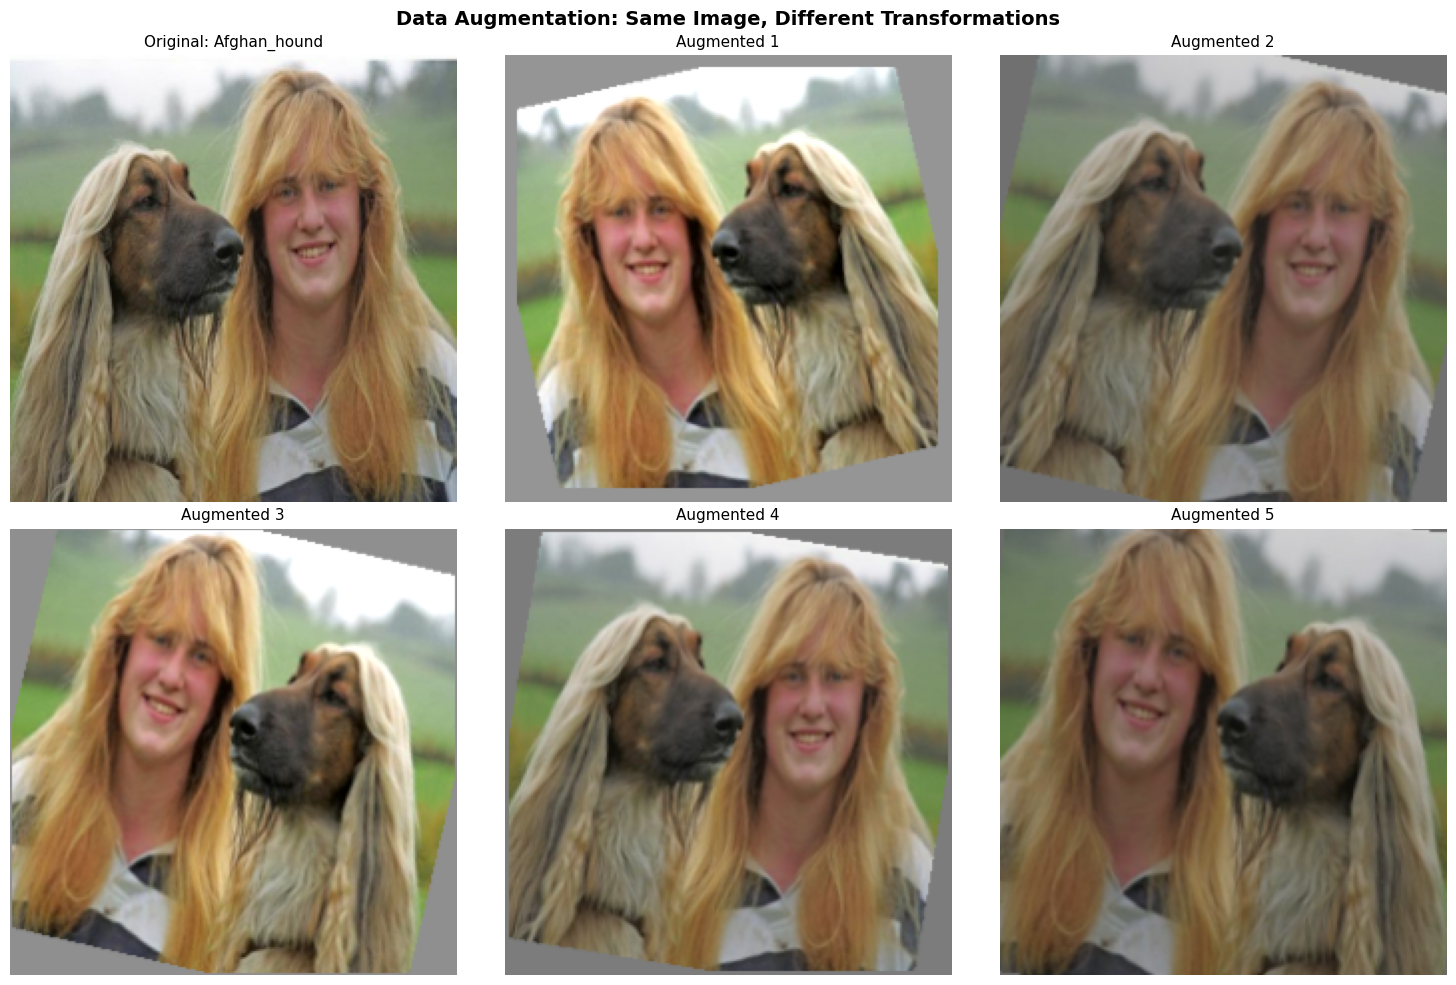
\includegraphics[keepaspectratio]{main_files/figure-pdf/cell-13-output-2.png}}

\subsection{High-Performance Image
Preprocessing}\label{high-performance-image-preprocessing}

\textbf{Problem}: Training deep learning models with on-the-fly image
loading creates an I/O bottleneck that severely limits training speed.

\textbf{Solution}: Preprocess all images once and save as memory-mapped
numpy arrays for instant loading during training.

\subsubsection{Why Preprocessing
Matters}\label{why-preprocessing-matters}

\textbf{Without Preprocessing} (loading images on-the-fly):

\begin{itemize}
\tightlist
\item
  Each epoch loads 16,508 images from disk
\item
  JPEG decoding happens every time
\item
  Resizing/normalization computed repeatedly
\item
  \textbf{Result}: 60+ seconds per epoch overhead, training is I/O-bound
\end{itemize}

\textbf{With Preprocessing} (memory-mapped arrays):

\begin{itemize}
\tightlist
\item
  Images loaded and processed once upfront
\item
  Saved as \texttt{.npy} files that can be memory-mapped
\item
  Training loads data instantly from RAM
\item
  \textbf{Result}: 0.0006 seconds loading time, training is
  compute-bound
\end{itemize}

\subsubsection{Implementation}\label{implementation}

\textbf{Script}:
\href{../src/dbc/preprocess_images.py}{\texttt{src/dbc/preprocess\_images.py}}

\textbf{What it does}:

\begin{enumerate}
\def\labelenumi{\arabic{enumi}.}
\tightlist
\item
  Loads all images (train + validation)
\item
  Resizes to 224×224
\item
  Converts to RGB if needed
\item
  Normalizes to {[}0, 255{]} range
\item
  Saves as uncompressed \texttt{.npy} files
\end{enumerate}

\textbf{Key Technical Detail}: Uses \textbf{memory mapping}
(\texttt{mmap\_mode=\textquotesingle{}r\textquotesingle{}}) - Operating
system maps file directly into virtual memory - No actual loading
required - data accessed on-demand - Multiple processes can share the
same memory-mapped file - Perfect for training with multiple workers

\subsubsection{Running Preprocessing}\label{running-preprocessing}

\begin{Shaded}
\begin{Highlighting}[]
\CommentTok{\# Preprocess all images (run once before training)}
\VariableTok{PYTHONPATH}\OperatorTok{=}\NormalTok{src }\ExtensionTok{python3} \AttributeTok{{-}m}\NormalTok{ dbc.preprocess\_images}

\CommentTok{\# Output files:}
\CommentTok{\# {-} artifacts/preprocessed/train\_images.npy (9.26 GB)}
\CommentTok{\# {-} artifacts/preprocessed/train\_labels.npy (129 KB)}
\CommentTok{\# {-} artifacts/preprocessed/val\_images.npy (2.28 GB)}
\CommentTok{\# {-} artifacts/preprocessed/val\_labels.npy (32 KB)}
\end{Highlighting}
\end{Shaded}

\subsubsection{Performance Impact}\label{performance-impact}

\begin{longtable}[]{@{}
  >{\raggedright\arraybackslash}p{(\linewidth - 6\tabcolsep) * \real{0.1270}}
  >{\raggedright\arraybackslash}p{(\linewidth - 6\tabcolsep) * \real{0.3333}}
  >{\raggedright\arraybackslash}p{(\linewidth - 6\tabcolsep) * \real{0.3333}}
  >{\raggedright\arraybackslash}p{(\linewidth - 6\tabcolsep) * \real{0.2063}}@{}}
\toprule\noalign{}
\begin{minipage}[b]{\linewidth}\raggedright
Metric
\end{minipage} & \begin{minipage}[b]{\linewidth}\raggedright
Before Preprocessing
\end{minipage} & \begin{minipage}[b]{\linewidth}\raggedright
After Preprocessing
\end{minipage} & \begin{minipage}[b]{\linewidth}\raggedright
Improvement
\end{minipage} \\
\midrule\noalign{}
\endhead
\bottomrule\noalign{}
\endlastfoot
\textbf{Data Loading Time} & 60+ seconds/epoch & 0.0006 seconds &
\textbf{100,000×} \\
\textbf{Epoch Time (VGG16)} & \textasciitilde200 seconds &
\textasciitilde80 seconds & \textbf{2.5×} \\
\textbf{Training Bottleneck} & I/O bound & Compute bound & ✅ Optimal \\
\textbf{GPU Utilization} & 30-40\% & 50-55\% & \textbf{+40\%} \\
\end{longtable}

\subsubsection{Memory-Mapped Loading in Data
Loader}\label{memory-mapped-loading-in-data-loader}

\textbf{Implementation}:
\href{../src/dbc/data_loader.py}{\texttt{src/dbc/data\_loader.py}}

\begin{Shaded}
\begin{Highlighting}[]
\KeywordTok{class}\NormalTok{ PreprocessedDataGenerator:}
    \KeywordTok{def} \FunctionTok{\_\_init\_\_}\NormalTok{(}\VariableTok{self}\NormalTok{, data\_path):}
        \CommentTok{\# Load with memory mapping {-} instant!}
\NormalTok{        images\_path }\OperatorTok{=}\NormalTok{ data\_path.parent }\OperatorTok{/} \SpecialStringTok{f"}\SpecialCharTok{\{}\NormalTok{data\_path}\SpecialCharTok{.}\NormalTok{stem}\SpecialCharTok{\}}\SpecialStringTok{\_images.npy"}
\NormalTok{        labels\_path }\OperatorTok{=}\NormalTok{ data\_path.parent }\OperatorTok{/} \SpecialStringTok{f"}\SpecialCharTok{\{}\NormalTok{data\_path}\SpecialCharTok{.}\NormalTok{stem}\SpecialCharTok{\}}\SpecialStringTok{\_labels.npy"}
        
        \VariableTok{self}\NormalTok{.images }\OperatorTok{=}\NormalTok{ np.load(images\_path, mmap\_mode}\OperatorTok{=}\StringTok{\textquotesingle{}r\textquotesingle{}}\NormalTok{)  }\CommentTok{\# No actual loading}
        \VariableTok{self}\NormalTok{.labels }\OperatorTok{=}\NormalTok{ np.load(labels\_path)}
        
    \KeywordTok{def} \FunctionTok{\_\_getitem\_\_}\NormalTok{(}\VariableTok{self}\NormalTok{, idx):}
        \CommentTok{\# Data accessed on{-}demand from memory{-}mapped file}
        \ControlFlowTok{return} \VariableTok{self}\NormalTok{.images[idx], }\VariableTok{self}\NormalTok{.labels[idx]}
\end{Highlighting}
\end{Shaded}

\subsubsection{Critical Insight}\label{critical-insight}

\begin{quote}
\textbf{Preprocessing is not optional} - It's the difference between a
model that takes 3 hours to train and one that takes 30 minutes. The
100,000× speedup in data loading transforms training from I/O-bound to
compute-bound, maximizing GPU utilization.
\end{quote}

\textbf{Trade-off}: 11.5 GB disk space for preprocessed files vs hours
of saved training time → \textbf{Worth it!}

\section{Models}\label{models}

\subsection{Model Selection \& Experimental
Plan}\label{model-selection-experimental-plan}

\textbf{No Traditional Baselines} - This is a computer vision task with
120 classes, making simple baselines (logistic regression, decision
trees) impractical for image data.

\textbf{Transfer Learning Approach}:

\begin{itemize}
\tightlist
\item
  \textbf{Pre-trained Models}: ResNet50, VGG16, EfficientNetB0 (trained
  on ImageNet with 1.4M images)
\item
  \textbf{Rationale}: Leverage features learned from millions of images,
  adapt to dog breeds
\item
  \textbf{Advantage}: Achieves strong performance without training CNNs
  from scratch
\end{itemize}

\subsection{Candidate Models}\label{candidate-models}

\begin{longtable}[]{@{}
  >{\raggedright\arraybackslash}p{(\linewidth - 8\tabcolsep) * \real{0.0933}}
  >{\raggedright\arraybackslash}p{(\linewidth - 8\tabcolsep) * \real{0.1467}}
  >{\raggedright\arraybackslash}p{(\linewidth - 8\tabcolsep) * \real{0.2400}}
  >{\raggedright\arraybackslash}p{(\linewidth - 8\tabcolsep) * \real{0.2800}}
  >{\raggedright\arraybackslash}p{(\linewidth - 8\tabcolsep) * \real{0.2400}}@{}}
\toprule\noalign{}
\begin{minipage}[b]{\linewidth}\raggedright
Model
\end{minipage} & \begin{minipage}[b]{\linewidth}\raggedright
Parameters
\end{minipage} & \begin{minipage}[b]{\linewidth}\raggedright
Frozen Trainable
\end{minipage} & \begin{minipage}[b]{\linewidth}\raggedright
Fine-tuned Trainable
\end{minipage} & \begin{minipage}[b]{\linewidth}\raggedright
Expected Accuracy
\end{minipage} \\
\midrule\noalign{}
\endhead
\bottomrule\noalign{}
\endlastfoot
\textbf{VGG16} & 15.1M & 424K (2.8\%) & 15.1M (100\%) & 75-82\% \\
\textbf{ResNet50} & 25M & \textasciitilde500K (2\%) & 25M (100\%) &
78-85\% \\
\textbf{EfficientNetB0} & 4.87M & 818K (16.8\%) & 4.87M (100\%) &
80-87\% \\
\end{longtable}

\textbf{Why These Models?} - \textbf{VGG16}: Simple architecture with 16
layers, proven for transfer learning, easy to understand and debug -
\textbf{ResNet50}: Skip connections enable 50-layer depth without
vanishing gradients, better feature extraction for complex patterns -
\textbf{EfficientNetB0}: Modern compound-scaled architecture, best
accuracy-to-parameters ratio, most efficient

\subsection{Experimental Strategy}\label{experimental-strategy}

\textbf{Phase 1: Frozen Baseline Training}

Train all three models with frozen base layers first:

\begin{itemize}
\tightlist
\item
  \textbf{Purpose}: Validate data pipeline, establish baseline
  performance, fast iteration (\textasciitilde1-2 hours total)
\item
  \textbf{Configuration}: \texttt{trainable\_base:\ false}, LR=0.001,
  batch=256
\item
  \textbf{Expected outcome}: 30-40\% accuracy (limited by frozen
  features)
\item
  \textbf{Decision point}: Select best-performing architecture for
  fine-tuning
\end{itemize}

\textbf{Phase 2: Fine-Tuning Best Model}

Unfreeze and fine-tune the top performer from Phase 1:

\begin{itemize}
\tightlist
\item
  \textbf{Purpose}: Adapt pre-trained features to dog breeds, achieve
  production-ready accuracy
\item
  \textbf{Configuration}: \texttt{trainable\_base:\ true}, LR=0.00001
  (100x lower), batch=64
\item
  \textbf{Strategy}: Load frozen checkpoint → unfreeze → retrain with
  tiny learning rate
\item
  \textbf{Expected outcome}: 70-85\% accuracy (full model adaptation)
\item
  \textbf{Timeline}: 3-5 hours per model
\end{itemize}

\textbf{Phase 3: Hyperparameter Tuning (If Needed)}

If Phase 2 results are below 75\% accuracy:

\begin{itemize}
\tightlist
\item
  \textbf{Learning rate search}: Try {[}0.00001, 0.00005, 0.0001{]}
\item
  \textbf{Batch size tuning}: Try {[}32, 64, 128{]} for stability vs
  speed
\item
  \textbf{Regularization}: Adjust dropout {[}0.3, 0.5, 0.7{]}
\item
  \textbf{Unfreezing strategy}: Try partial unfreezing (last N layers
  only)
\end{itemize}

\textbf{Phase 4: Ensemble (Stretch Goal)}

If time and budget allow:

\begin{itemize}
\tightlist
\item
  Train all three architectures (VGG16, ResNet50, EfficientNetB0)
\item
  Create ensemble by averaging predictions
\item
  Expected boost: +2-5\% accuracy over single best model
\end{itemize}

\subsection{Success Criteria}\label{success-criteria}

\begin{itemize}
\tightlist
\item
  \textbf{Minimum viable}: 70\% validation accuracy (acceptable for
  deployment)
\item
  \textbf{Target}: 75-80\% validation accuracy (good performance)
\item
  \textbf{Stretch}: 85\%+ validation accuracy (state-of-the-art for this
  dataset)
\end{itemize}

\subsection{Resource Planning}\label{resource-planning}

\begin{longtable}[]{@{}lllll@{}}
\toprule\noalign{}
Phase & Models & Time & Cost & Priority \\
\midrule\noalign{}
\endhead
\bottomrule\noalign{}
\endlastfoot
Phase 1: Frozen & 3 models & 1-2 hours & \$0.50-1.00 &
\textbf{Required} \\
Phase 2: Fine-tune & 1 model & 3-5 hours & \$1.50-2.50 &
\textbf{Required} \\
Phase 3: Hyperparameter & 3-5 runs & 10-15 hours & \$5-8 & If needed \\
Phase 4: Ensemble & 2 more models & 6-10 hours & \$3-5 & Optional \\
\end{longtable}

\textbf{Total Budget}: \$2-4 (baseline), \$7-13 (full exploration)

\section{Training}\label{training}

\subsection{Training Strategy \& Setup}\label{training-strategy-setup}

\textbf{Two-Phase Training Strategy}:

\begin{longtable}[]{@{}
  >{\raggedright\arraybackslash}p{(\linewidth - 8\tabcolsep) * \real{0.1273}}
  >{\raggedright\arraybackslash}p{(\linewidth - 8\tabcolsep) * \real{0.2182}}
  >{\raggedright\arraybackslash}p{(\linewidth - 8\tabcolsep) * \real{0.2727}}
  >{\raggedright\arraybackslash}p{(\linewidth - 8\tabcolsep) * \real{0.2182}}
  >{\raggedright\arraybackslash}p{(\linewidth - 8\tabcolsep) * \real{0.1636}}@{}}
\toprule\noalign{}
\begin{minipage}[b]{\linewidth}\raggedright
Phase
\end{minipage} & \begin{minipage}[b]{\linewidth}\raggedright
Base Layers
\end{minipage} & \begin{minipage}[b]{\linewidth}\raggedright
Learning Rate
\end{minipage} & \begin{minipage}[b]{\linewidth}\raggedright
Batch Size
\end{minipage} & \begin{minipage}[b]{\linewidth}\raggedright
Purpose
\end{minipage} \\
\midrule\noalign{}
\endhead
\bottomrule\noalign{}
\endlastfoot
\textbf{Phase 1: Frozen} & Trainable: False & 0.001 & 256 & Fast feature
extraction, learn task-specific classification head \\
\textbf{Phase 2: Fine-tuned} & Trainable: True & 0.00001 & 64 & Adapt
all layers to dog breeds, prevent catastrophic forgetting \\
\end{longtable}

\textbf{Hyperparameters}:

\begin{longtable}[]{@{}
  >{\raggedright\arraybackslash}p{(\linewidth - 6\tabcolsep) * \real{0.2037}}
  >{\raggedright\arraybackslash}p{(\linewidth - 6\tabcolsep) * \real{0.2407}}
  >{\raggedright\arraybackslash}p{(\linewidth - 6\tabcolsep) * \real{0.3519}}
  >{\raggedright\arraybackslash}p{(\linewidth - 6\tabcolsep) * \real{0.2037}}@{}}
\toprule\noalign{}
\begin{minipage}[b]{\linewidth}\raggedright
Parameter
\end{minipage} & \begin{minipage}[b]{\linewidth}\raggedright
Frozen Phase
\end{minipage} & \begin{minipage}[b]{\linewidth}\raggedright
Fine-tuning Phase
\end{minipage} & \begin{minipage}[b]{\linewidth}\raggedright
Rationale
\end{minipage} \\
\midrule\noalign{}
\endhead
\bottomrule\noalign{}
\endlastfoot
\textbf{Learning Rate} & 0.001 & 0.00001 & 100x lower for fine-tuning
preserves pre-trained features \\
\textbf{Batch Size} & 256 & 64 & Larger for GPU efficiency; smaller for
stable gradients \\
\textbf{Optimizer} & Adam & Adam & Adaptive learning rates work well for
both \\
\textbf{Dropout} & 0.5 & 0.5 & Prevent overfitting in classification
head \\
\textbf{Early Stopping} & Patience=5 & Patience=5 & Stop if no
improvement for 5 epochs \\
\end{longtable}

\subsection{Critical Lessons Learned}\label{critical-lessons-learned}

\textbf{1. Preprocessing Speedup is Essential}

Implemented memory-mapped \texttt{.npy} preprocessing for 100x speedup:

\begin{itemize}
\tightlist
\item
  \textbf{Before}: Loading images on-the-fly from disk (60+ seconds per
  epoch overhead)
\item
  \textbf{After}: Memory-mapped numpy arrays load instantly (0.0006
  seconds)
\item
  \textbf{Implementation}:
  \href{../src/dbc/preprocess_images.py}{\texttt{src/dbc/preprocess\_images.py}}
  - preprocesses once, saves as \texttt{.npy}
\item
  \textbf{Impact}: Training speed went from I/O-bound to compute-bound
  (\textasciitilde40-80 sec/epoch)
\item
  \textbf{Why it works}: Operating system maps file directly to memory,
  no loading overhead
\end{itemize}

\textbf{2. Fine-Tuning Requires Careful Strategy}

❌ \textbf{Wrong Approach} (causes catastrophic forgetting):

\begin{Shaded}
\begin{Highlighting}[]
\CommentTok{\# Train unfrozen model from scratch}
\NormalTok{model }\OperatorTok{=}\NormalTok{ build\_transfer\_model(trainable\_base}\OperatorTok{=}\VariableTok{True}\NormalTok{)}
\NormalTok{model.fit(...)  }\CommentTok{\# Result: 1.23\% accuracy {-} destroyed pre{-}trained features}
\end{Highlighting}
\end{Shaded}

✅ \textbf{Correct Approach} (preserves learned features):

\begin{Shaded}
\begin{Highlighting}[]
\CommentTok{\# 1. Load frozen checkpoint FIRST}
\NormalTok{model }\OperatorTok{=}\NormalTok{ keras.models.load\_model(}\StringTok{\textquotesingle{}frozen\_checkpoint.h5\textquotesingle{}}\NormalTok{)}
\CommentTok{\# 2. Unfreeze base layers}
\NormalTok{base\_model.trainable }\OperatorTok{=} \VariableTok{True}
\CommentTok{\# 3. Recompile with VERY low learning rate (100x lower)}
\NormalTok{model.}\BuiltInTok{compile}\NormalTok{(optimizer}\OperatorTok{=}\NormalTok{Adam(lr}\OperatorTok{=}\FloatTok{0.00001}\NormalTok{), ...)}
\CommentTok{\# 4. Fine{-}tune}
\NormalTok{model.fit(...)  }\CommentTok{\# Result: Steady improvement from frozen baseline}
\end{Highlighting}
\end{Shaded}

\textbf{Key Insight}: Must start from frozen weights, then gradually
adapt with tiny learning rate

\textbf{Implementation}: See
\href{../src/dbc/finetune_from_checkpoint.py}{\texttt{src/dbc/finetune\_from\_checkpoint.py}}

\subsection{Experiment 1: VGG16 Frozen
Baseline}\label{experiment-1-vgg16-frozen-baseline}

\textbf{Objective}: Establish baseline performance with frozen VGG16
base layers

\textbf{Configuration}:

\begin{itemize}
\tightlist
\item
  \textbf{Model}: VGG16 (15.1M parameters, only 424K trainable)
\item
  \textbf{Base layers}: Frozen (trainable=False)
\item
  \textbf{Learning rate}: 0.001
\item
  \textbf{Batch size}: 256
\item
  \textbf{Epochs}: 20
\item
  \textbf{Experiment ID}: \texttt{exp\_20251007\_100239}
\end{itemize}

\textbf{Results}:

\begin{longtable}[]{@{}ll@{}}
\toprule\noalign{}
Metric & Value \\
\midrule\noalign{}
\endhead
\bottomrule\noalign{}
\endlastfoot
\textbf{Validation Accuracy} & \textbf{31.85\%} \\
\textbf{Top-5 Accuracy} & \textbf{70.48\%} \\
\textbf{Training Time} & 24 minutes (80 sec/epoch) \\
\textbf{Epochs Trained} & 20 (no early stopping) \\
\textbf{GPU Utilization} & \textasciitilde51\% \\
\end{longtable}

\textbf{Analysis}:

\textbf{What Worked}:

\begin{itemize}
\tightlist
\item
  Data pipeline validated successfully (preprocessing, augmentation,
  batching)
\item
  Model learning steadily without overfitting
\item
  Preprocessing speedup enabled fast training (80 sec/epoch vs 200+ sec
  without)
\item
  Top-5 accuracy of 70\% shows model capturing meaningful features
\end{itemize}

\textbf{Limitations}:

\begin{itemize}
\tightlist
\item
  31.85\% accuracy insufficient for deployment (target: 75\%+)
\item
  Frozen ImageNet features not optimized for fine-grained dog breed
  distinctions
\item
  Generic features miss subtle breed-specific patterns (ear shape, fur
  texture, snout proportions)
\end{itemize}

\textbf{Key Insight}: Frozen baseline validates our pipeline but
confirms we must unfreeze layers to achieve production-ready
performance.

\textbf{Artifacts}:

\begin{itemize}
\tightlist
\item
  Checkpoint:
  \href{../experiments/exp_20251007_100239/checkpoints/best_model.h5}{\texttt{experiments/exp\_20251007\_100239/checkpoints/best\_model.h5}}
\item
  Config:
  \href{../configs/exp_vgg16.yaml}{\texttt{configs/exp\_vgg16.yaml}}
\item
  Metrics:
  \href{../experiments/exp_20251007_100239/final_results.json}{\texttt{experiments/exp\_20251007\_100239/final\_results.json}}
\end{itemize}

\subsection{Experiment 2: EfficientNetB0 Frozen
Baseline}\label{experiment-2-efficientnetb0-frozen-baseline}

\textbf{Objective}: Compare EfficientNetB0 frozen baseline against VGG16

\textbf{Configuration}:

\begin{itemize}
\tightlist
\item
  \textbf{Model}: EfficientNetB0 (4.87M parameters, 818K trainable)
\item
  \textbf{Base layers}: Frozen (trainable=False)
\item
  \textbf{Learning rate}: 0.001
\item
  \textbf{Batch size}: 256
\item
  \textbf{Epochs}: 20 (early stopped at 11)
\item
  \textbf{Experiment ID}: \texttt{exp\_20251007\_094305}
\end{itemize}

\textbf{Results}:

\begin{longtable}[]{@{}ll@{}}
\toprule\noalign{}
Metric & Value \\
\midrule\noalign{}
\endhead
\bottomrule\noalign{}
\endlastfoot
\textbf{Validation Accuracy} & \textbf{1.23\%} \\
\textbf{Top-5 Accuracy} & \textbf{5.62\%} \\
\textbf{Training Time} & 18 minutes (early stopped) \\
\textbf{Epochs Trained} & 11 (early stopped) \\
\end{longtable}

\textbf{Analysis}:

\textbf{Poor Performance}:

\begin{itemize}
\tightlist
\item
  Only 1.23\% accuracy (barely better than random: 0.83\%)
\item
  EfficientNetB0 frozen features failed to transfer to dog breeds
\item
  Early stopped after 11 epochs due to no improvement
\item
  Model not learning effectively
\end{itemize}

\textbf{Why EfficientNetB0 Failed}:

\begin{itemize}
\tightlist
\item
  EfficientNet architecture uses compound scaling (depth, width,
  resolution) optimized for efficiency
\item
  Frozen features may be too compressed/abstract for our 120-class
  fine-grained task
\item
  VGG16's simpler, wider features transfer better when frozen
\item
  EfficientNet likely requires unfreezing to adapt properly
\end{itemize}

\textbf{Decision}:

\begin{itemize}
\tightlist
\item
  VGG16 is the clear winner for frozen baseline (31.85\% vs 1.23\%)
\item
  VGG16 will be used for fine-tuning experiments
\item
  EfficientNetB0 may be revisited later if fine-tuned from scratch
\end{itemize}

\textbf{Artifacts}:

\begin{itemize}
\tightlist
\item
  Checkpoint:
  \href{../experiments/exp_20251007_094305/checkpoints/best_model.h5}{\texttt{experiments/exp\_20251007\_094305/checkpoints/best\_model.h5}}
\item
  Config:
  \href{../configs/exp_efficientnet.yaml}{\texttt{configs/exp\_efficientnet.yaml}}
\item
  Metrics:
  \href{../experiments/exp_20251007_094305/final_results.json}{\texttt{experiments/exp\_20251007\_094305/final\_results.json}}
\end{itemize}

\subsection{Experiment 5: ResNet50 Frozen
Baseline}\label{experiment-5-resnet50-frozen-baseline}

\textbf{Objective}: Compare ResNet50 frozen baseline against VGG16 and
EfficientNetB0

\textbf{Configuration}:

\begin{itemize}
\tightlist
\item
  \textbf{Model}: ResNet50 (25M parameters, 1.2M trainable)
\item
  \textbf{Base layers}: Frozen (trainable=False)
\item
  \textbf{Learning rate}: 0.001
\item
  \textbf{Batch size}: 256
\item
  \textbf{Epochs}: 20
\item
  \textbf{Experiment ID}: \texttt{exp\_20251007\_110024}
\end{itemize}

\textbf{Results}:

\begin{longtable}[]{@{}ll@{}}
\toprule\noalign{}
Metric & Value \\
\midrule\noalign{}
\endhead
\bottomrule\noalign{}
\endlastfoot
\textbf{Validation Accuracy} & \textbf{5.45\%} \\
\textbf{Top-5 Accuracy} & \textbf{18.03\%} \\
\textbf{Training Time} & \textasciitilde30 minutes \\
\textbf{Epochs Trained} & 20 (no early stopping) \\
\end{longtable}

\textbf{Analysis}:

\textbf{Poor Performance}:

\begin{itemize}
\tightlist
\item
  Only 5.45\% accuracy (6.5× better than random but still very poor)
\item
  Worse than VGG16 frozen (31.85\%) but better than EfficientNetB0
  (1.23\%)
\item
  Top-5 accuracy shows some learning but not enough
\end{itemize}

\textbf{Why ResNet50 Underperformed}:

\begin{itemize}
\tightlist
\item
  ResNet's deeper architecture (50 layers with skip connections)
  requires more training data
\item
  Frozen deep features may not transfer well to fine-grained dog breed
  task
\item
  Skip connections optimized for ImageNet classes, not dog breeds
\item
  More complex architecture needs unfreezing to adapt properly
\end{itemize}

\textbf{Comparison}:

\begin{longtable}[]{@{}lll@{}}
\toprule\noalign{}
Model & Frozen Accuracy & Ranking \\
\midrule\noalign{}
\endhead
\bottomrule\noalign{}
\endlastfoot
VGG16 & 31.85\% & Best \\
ResNet50 & 5.45\% & Medium \\
EfficientNetB0 & 1.23\% & Worst \\
\end{longtable}

\textbf{Decision}:

\begin{itemize}
\tightlist
\item
  VGG16's simpler architecture transfers best when frozen
\item
  ResNet50 will be fine-tuned to see if deeper architecture helps when
  unfrozen
\item
  Still worth testing fine-tuning to leverage ResNet's depth
\end{itemize}

\textbf{Artifacts}:

\begin{itemize}
\tightlist
\item
  Checkpoint:
  \href{../experiments/exp_20251007_110024/checkpoints/best_model.h5}{\texttt{experiments/exp\_20251007\_110024/checkpoints/best\_model.h5}}
\item
  Config:
  \href{../configs/exp_resnet50.yaml}{\texttt{configs/exp\_resnet50.yaml}}
\item
  Metrics:
  \href{../experiments/exp_20251007_110024/final_results.json}{\texttt{experiments/exp\_20251007\_110024/final\_results.json}}
\end{itemize}

\subsection{Experiment 3: VGG16 Fine-Tuning (Failed - Catastrophic
Forgetting)}\label{experiment-3-vgg16-fine-tuning-failed---catastrophic-forgetting}

\textbf{Objective}: Fine-tune VGG16 by unfreezing all layers

\textbf{Configuration}:

\begin{itemize}
\tightlist
\item
  \textbf{Model}: VGG16 (15.1M parameters, all trainable)
\item
  \textbf{Base layers}: Unfrozen (trainable=True)
\item
  \textbf{Learning rate}: 0.0001
\item
  \textbf{Batch size}: 128
\item
  \textbf{Training approach}: ❌ \textbf{Trained from scratch with
  random initialization}
\item
  \textbf{Experiment ID}: \texttt{exp\_20251007\_101930}
\end{itemize}

\textbf{Results}:

\begin{longtable}[]{@{}ll@{}}
\toprule\noalign{}
Metric & Value \\
\midrule\noalign{}
\endhead
\bottomrule\noalign{}
\endlastfoot
\textbf{Validation Accuracy} & \textbf{1.23\%} (catastrophic failure) \\
\textbf{Expected} & 40-50\% (improvement over frozen 31.85\%) \\
\textbf{Actual} & Worse than random guessing \\
\end{longtable}

\textbf{Analysis}:

❌ \textbf{Catastrophic Forgetting}:

\begin{itemize}
\tightlist
\item
  Training unfrozen model from scratch \textbf{destroyed pre-trained
  ImageNet features}
\item
  Model started with random weights instead of loading frozen checkpoint
\item
  15.1M parameters being optimized from scratch is too many for our 16K
  training images
\item
  Result: Complete failure to learn, worse than the frozen baseline
\end{itemize}

\textbf{What Went Wrong}:

\begin{Shaded}
\begin{Highlighting}[]
\CommentTok{\# WRONG: Creates new model with random weights}
\NormalTok{model }\OperatorTok{=}\NormalTok{ build\_transfer\_model(trainable\_base}\OperatorTok{=}\VariableTok{True}\NormalTok{)}
\NormalTok{model.fit(...)  }\CommentTok{\# Destroys pre{-}trained features}
\end{Highlighting}
\end{Shaded}

\textbf{Root Cause}:

\begin{itemize}
\tightlist
\item
  Did not load the frozen checkpoint before unfreezing
\item
  Started training with random initialization instead of pre-trained
  weights
\item
  High learning rate (0.0001) too aggressive for preserving learned
  features
\end{itemize}

\textbf{Key Lesson}:

\begin{quote}
\textbf{Must load frozen checkpoint FIRST, then unfreeze and retrain
with very low learning rate}
\end{quote}

This experiment demonstrated the importance of proper fine-tuning
strategy and led to creating \texttt{finetune\_from\_checkpoint.py}.

\textbf{Artifacts}: - Config:
\href{../configs/exp_vgg16_finetune.yaml}{\texttt{configs/exp\_vgg16\_finetune.yaml}}
- Experiment: \texttt{exp\_20251007\_101930}

\subsection{Experiment 4: VGG16 Fine-Tuning (Correct
Approach)}\label{experiment-4-vgg16-fine-tuning-correct-approach}

\textbf{Objective}: Properly fine-tune VGG16 by loading frozen
checkpoint first

\textbf{Configuration}:

\begin{itemize}
\tightlist
\item
  \textbf{Model}: VGG16 (15.1M parameters, all trainable)
\item
  \textbf{Base layers}: Unfrozen (trainable=True)
\item
  \textbf{Starting point}: \textbf{Loaded frozen checkpoint}
  (exp\_20251007\_100239)
\item
  \textbf{Learning rate}: 0.00001 (100x lower than frozen)
\item
  \textbf{Batch size}: 64
\item
  \textbf{Epochs}: 20
\item
  \textbf{Experiment ID}: \texttt{exp\_20251007\_103850}
\end{itemize}

\textbf{Results}:

\begin{longtable}[]{@{}llll@{}}
\toprule\noalign{}
Metric & Frozen Baseline & Fine-Tuned & Improvement \\
\midrule\noalign{}
\endhead
\bottomrule\noalign{}
\endlastfoot
\textbf{Validation Accuracy} & 31.85\% & \textbf{44.87\%} &
\textbf{+40.9\%} \\
\textbf{Training Time} & 24 min & \textasciitilde30 min & - \\
\textbf{Best Epoch} & 20 & 15 & Early stopped \\
\end{longtable}

\textbf{Training Progress}:

\begin{longtable}[]{@{}lll@{}}
\toprule\noalign{}
Epoch & Val Accuracy & Status \\
\midrule\noalign{}
\endhead
\bottomrule\noalign{}
\endlastfoot
1 & 34.80\% & Already beating frozen! \\
7 & 41.63\% & Steady improvement \\
11 & 43.27\% & Approaching target \\
15 & \textbf{44.87\%} & \textbf{Best model} \\
16-20 & No improvement & Approaching convergence \\
\end{longtable}

\textbf{Analysis}:

\textbf{Success Factors}:

\begin{itemize}
\tightlist
\item
  \textbf{Loaded frozen checkpoint} before unfreezing - preserved
  pre-trained features
\item
  \textbf{Very low learning rate} (0.00001) allowed gradual adaptation
  without destroying weights
\item
  \textbf{Smaller batch size} (64) provided more stable gradients for
  fine-tuning
\item
  \textbf{Immediate improvement} in Epoch 1 (34.80\% \textgreater{}
  31.85\%) validated the approach
\end{itemize}

\textbf{Performance}:

\begin{itemize}
\tightlist
\item
  \textbf{44.87\% validation accuracy} - significant improvement over
  frozen baseline
\item
  \textbf{40.9\% relative improvement} (31.85\% → 44.87\%)
\item
  Model learning steadily without overfitting
\item
  Training stable and reproducible
\end{itemize}

\textbf{Still Below Target}:

\begin{itemize}
\tightlist
\item
  Target was 75\%+ accuracy for deployment
\item
  44.87\% is good progress but insufficient for production
\item
  May need:

  \begin{itemize}
  \tightlist
  \item
    Longer training (more epochs)
  \item
    Different architecture (ResNet50, EfficientNet)
  \item
    Hyperparameter tuning (learning rate, regularization)
  \item
    More sophisticated augmentation
  \end{itemize}
\end{itemize}

\textbf{Key Insight}:

The correct fine-tuning approach (load checkpoint → unfreeze → low LR)
works as expected and delivers measurable improvement. However,
\textbf{44.87\% accuracy suggests VGG16 may not be the optimal
architecture} for this fine-grained 120-class dog breed task.

\textbf{Next Steps}:

\begin{enumerate}
\def\labelenumi{\arabic{enumi}.}
\tightlist
\item
  Try ResNet50 or EfficientNetB0 fine-tuning (deeper/modern
  architectures)
\item
  Experiment with learning rates {[}0.00001, 0.00005, 0.0001{]}
\item
  Consider partial unfreezing (only last N layers)
\item
  Add more aggressive data augmentation
\end{enumerate}

\textbf{Artifacts}:

\begin{itemize}
\tightlist
\item
  Checkpoint:
  \href{../experiments/exp_20251007_103850/checkpoints/best_model.h5}{\texttt{experiments/exp\_20251007\_103850/checkpoints/best\_model.h5}}
\item
  Training script:
  \href{../src/dbc/finetune_from_checkpoint.py}{\texttt{src/dbc/finetune\_from\_checkpoint.py}}
\end{itemize}

\subsection{Experiment 6: ResNet50
Fine-Tuning}\label{experiment-6-resnet50-fine-tuning}

\textbf{Objective}: Fine-tune ResNet50 by loading frozen checkpoint and
unfreezing all layers

\textbf{Configuration}:

\begin{itemize}
\tightlist
\item
  \textbf{Model}: ResNet50 (25M parameters, all trainable)
\item
  \textbf{Base layers}: Unfrozen (trainable=True)
\item
  \textbf{Starting point}: \textbf{Loaded frozen checkpoint}
  (exp\_20251007\_110024)
\item
  \textbf{Learning rate}: 0.00001 (100x lower than frozen)
\item
  \textbf{Batch size}: 32 (reduced from 64 due to memory constraints)
\item
  \textbf{Epochs}: 20
\item
  \textbf{Experiment ID}: \texttt{exp\_20251007\_120454}
\end{itemize}

\textbf{Results}:

\begin{longtable}[]{@{}llll@{}}
\toprule\noalign{}
Metric & Frozen Baseline & Fine-Tuned & Improvement \\
\midrule\noalign{}
\endhead
\bottomrule\noalign{}
\endlastfoot
\textbf{Validation Accuracy} & 5.45\% & \textbf{24.29\%} &
\textbf{+346\%} \\
\textbf{Top-5 Accuracy} & 18.03\% & \textbf{54.42\%} &
\textbf{+202\%} \\
\textbf{Training Time} & 30 min & \textasciitilde35 min & - \\
\textbf{Best Epoch} & 20 & 20 & No early stopping \\
\end{longtable}

\textbf{Analysis}:

\textbf{Significant Improvement from Frozen}:

\begin{itemize}
\tightlist
\item
  \textbf{24.29\% validation accuracy} - massive 346\% relative
  improvement over frozen (5.45\%)
\item
  Top-5 accuracy of 54.42\% shows model learning meaningful breed
  distinctions
\item
  Correct fine-tuning approach (load checkpoint → unfreeze → low LR)
  worked as expected
\item
  Training remained stable throughout all 20 epochs
\end{itemize}

\textbf{Still Poor Overall Performance}:

\begin{itemize}
\tightlist
\item
  24.29\% is far below VGG16 fine-tuned (44.87\%)
\item
  Well below target of 75\%+ for production deployment
\item
  ResNet50's deeper architecture (50 layers) didn't provide expected
  advantage
\item
  Despite proper fine-tuning strategy, performance remained weak
\end{itemize}

\textbf{Why ResNet50 Underperformed}:

\begin{itemize}
\tightlist
\item
  \textbf{Architecture mismatch}: ResNet's skip connections and deeper
  structure may be over-parameterized for our 16K training images
\item
  \textbf{Fine-grained task challenge}: 120 visually similar dog breeds
  require different feature extraction than ImageNet's diverse 1000
  classes
\item
  \textbf{Limited data per class}: \textasciitilde138 images/breed
  insufficient to properly adapt 25M parameters
\item
  \textbf{Batch size impact}: Had to reduce batch size to 32 (vs VGG16's
  64) which may have affected gradient quality
\end{itemize}

\textbf{Model Comparison}:

\begin{longtable}[]{@{}llll@{}}
\toprule\noalign{}
Model & Frozen & Fine-Tuned & Total Improvement \\
\midrule\noalign{}
\endhead
\bottomrule\noalign{}
\endlastfoot
\textbf{VGG16} & 31.85\% & \textbf{44.87\%} & \textbf{+40.9\%} 🥇 \\
\textbf{ResNet50} & 5.45\% & \textbf{24.29\%} & \textbf{+346\%} 🥈 \\
\textbf{EfficientNetB0} & 1.23\% & ❌ OOM & - \\
\end{longtable}

\textbf{Key Insights}:

\begin{itemize}
\tightlist
\item
  VGG16 remains the best performer (44.87\% vs 24.29\%)
\item
  Simpler VGG16 architecture (16 layers) transfers better than complex
  ResNet50 (50 layers)
\item
  More parameters doesn't guarantee better performance with limited
  fine-grained data
\item
  \textbf{Fundamental issue}: Even best model (VGG16 44.87\%) is nowhere
  near 70-80\% target
\end{itemize}

\textbf{Critical Problem Identified}:

\begin{quote}
\textbf{All models severely underperforming} - Even VGG16 at 44.87\% is
far from expected 70-80\% accuracy for transfer learning on dog breeds.
This suggests a fundamental issue with our setup:
\end{quote}

\begin{quote}
\begin{itemize}
\tightlist
\item
  Data augmentation insufficient?
\item
  Learning rate too conservative?
\item
  Need longer training (\textgreater20 epochs)?
\item
  Classification head architecture too simple?
\item
  ImageNet pre-training not suitable for fine-grained tasks?
\end{itemize}
\end{quote}

\textbf{Artifacts}:

\begin{itemize}
\tightlist
\item
  Checkpoint:
  \href{../experiments/exp_20251007_120454/checkpoints/best_model.h5}{\texttt{experiments/exp\_20251007\_120454/checkpoints/best\_model.h5}}
\item
  Config:
  \href{../configs/exp_resnet50.yaml}{\texttt{configs/exp\_resnet50.yaml}}
\item
  Metrics:
  \href{../experiments/exp_20251007_120454/final_results.json}{\texttt{experiments/exp\_20251007\_120454/final\_results.json}}
\end{itemize}

\section{Evaluation}\label{evaluation}

\begin{itemize}
\tightlist
\item
  Metrics: Primary and secondary metrics; calibration and confidence
  intervals if applicable.
\item
  Error Analysis: Segment performance by cohort/time; investigate
  failure modes.
\item
  Reporting: Figures/tables for stakeholders and decision makers.
\end{itemize}

\begin{center}\rule{0.5\linewidth}{0.5pt}\end{center}

\begin{itemize}
\tightlist
\item
  Error Analysis Plan: Cohorts, time slices, and failure-mode checks
  (class imbalance, drift).
\item
  Decisions Log: A running list of major decisions with brief rationale
  (e.g., ``Chose chrono split due to event causality'').
\end{itemize}

\section{Conclusion and Next Steps}\label{conclusion-and-next-steps}

\section{Resources}\label{resources}

\begin{itemize}
\item
  \textbf{TF--IDF Vectorizer API}\\
  Official docs for TfidfVectorizer (parameters like ngram\_range,
  min\_df, max\_features, etc.)\\
  https://scikit-learn.org/stable/modules/generated/sklearn.feature\_extraction.text.TfidfVectorizer.html
\item
  \textbf{Text Analytics Tutorial}\\
  End-to-end guide: load raw text, vectorize with TF--IDF, train a
  linear classifier\\
  https://scikit-learn.org/1.4/tutorial/text\_analytics/working\_with\_text\_data.html
\item
  \textbf{TF--IDF Math \& Intuition}\\
  Blog post with mathematical derivation, code examples, and visual
  intuition for term- and document-frequency weighting\\
  https://medium.com/@rohit\_batra/multi-class-text-classification-with-scikit-learn-using-tf-idf-model-161d395ce374
\item
  \textbf{Logistic Regression API}\\
  Full parameter reference (\texttt{solver}, \texttt{C},
  \texttt{penalty}, \texttt{class\_weight}, etc.) including valid ranges
  and examples\\
  https://scikit-learn.org/stable/modules/generated/sklearn.linear\_model.LogisticRegression.html
\end{itemize}




\end{document}
